% ============================================================================
% BOLUM 4: DENEYLER
% ============================================================================
% 2026-10-04 (LeCun turu): EN 04_experiments.tex ile cumle duzeyinde esitlendi.
% Sira: A mutlak gurbuzluk -> B protokoller ve ozdeslik -> C kaynak etkisi ->
% D ayarlar arasi + yayilim/temiz fark sekli -> E standart hedefler ve dis havuz
% -> F secim kurali -> G uc okuma (gradyan, dikkat, TGR) -> H varyans kaynaklari.
% Karantina literalleri (eski Tablo 2 alt blogu, Tablo 3 dipnotu) cikarildi.
% Her sayi results/C1_REFERANS_FOYU.md'den.
\section{Deneyler}
\label{sec:experiments}

% ----------------------------------------------------------------------------
% A. Gurbuzluk karsilastirmasi
% ----------------------------------------------------------------------------
\subsection{Gürbüzlük Karşılaştırması}
\label{subsec:robustness}

Tablo~\ref{tab:main_results} mutlak gürbüzlüğü vermektedir. Bu çalışmada eğitilen modellere ait her hücre, mimari başına üç bağımsız eğitim koşusunun ortalaması ve bu koşular üzerindeki standart sapmadır; her koşu 10.000 örneklik tam test kümesinde değerlendirilmiştir.

\begin{table}[!t]
\centering
\caption{CIFAR-10'da ana gürbüzlük sonuçları ($\eps = 8/255$); mimari başına üç bağımsız eğitim koşusu üzerinden ortalama$\pm$std. AA, standart takımla AutoAttack anlamına gelmektedir.}
\label{tab:main_results}
\scriptsize
\setlength{\tabcolsep}{2pt}
\begin{tabular}{lcccccc}
\toprule
\textbf{Model} & \textbf{Savunma} & \textbf{Param.} & \textbf{Temiz} & \textbf{FGSM} & \textbf{PGD-10} & \textbf{AA} \\
\midrule
\multicolumn{7}{l}{\textit{CNN Modelleri}} \\
ResNet-18 & Yok & 11,2M & 95,25$\pm$0,15 & 40,29$\pm$1,77 & 0,03$\pm$0,03 & -- \\
ResNet-18 & AT & 11,2M & 85,78$\pm$0,36 & 53,46$\pm$0,08 & 44,11$\pm$0,50 & \textbf{37,93$\pm$0,14} \\
WRN-28-10 & AT$^\dagger$ & 36,5M & 89,48 & 70,91 & 66,92 & 62,76 \\
\midrule
\multicolumn{7}{l}{\textit{Görü Dönüştürücüsü Modelleri}} \\
ViT-Tiny & Yok & 5,7M & 80,09$\pm$0,60 & 6,10$\pm$1,47 & 0,05$\pm$0,05 & -- \\
ViT-Tiny & AT & 5,7M & 73,53$\pm$0,55 & 36,31$\pm$0,42 & 32,69$\pm$0,22 & \textbf{29,14$\pm$0,40} \\
\bottomrule
\multicolumn{7}{l}{\scriptsize $^\dagger$Gowal vd.'nin~\cite{gowal2020uncovering} RobustBench~\cite{croce2021robustbench} üzerinden dağıtılan gürbüz kontrol}\\
\multicolumn{7}{l}{\scriptsize \phantom{$^\dagger$}noktası; tek harici kontrol noktası olduğundan standart sapma yoktur.}\\
\multicolumn{7}{l}{\scriptsize \phantom{$^\dagger$}Temiz/FGSM/PGD-10: yerel tam test değerlendirmeleri; AA: RobustBench'in}\\
\multicolumn{7}{l}{\scriptsize \phantom{$^\dagger$}raporladığı değer (bu model üzerinde AutoAttack yeniden koşulmamıştır).}
\end{tabular}
\end{table}

CNN her saldırı altında \emph{mutlak} bir gürbüzlük üstünlüğü taşımaktadır: ResNet-18 AT, AutoAttack altında $\%37{,}93\pm0{,}14$ gürbüz doğruluğa ulaşırken ViT-Tiny AT $\%29{,}14\pm0{,}40$'ta kalmaktadır. Bir çiftin iki modeli de aynı 10.000 örnekte, örnek bazında kayıtla değerlendirildiğinden her koşu içinde McNemar'ın eşleştirilmiş testi uygulanabilmekte ve bu test üç çiftte de CNN lehine sonuç vermektedir (AutoAttack altında $p < 2\times10^{-84}$, PGD-10 altında $p < 2\times10^{-120}$). Çekişmeli eğitilmiş çiftte tohum düzeyindeki değişim raporlanan hiçbir doğrulukta 0,55 puanı aşmamaktadır; dolayısıyla sıralama koşudan koşuya gürültü değildir. CNN ayrıca daha yüksek bir temiz doğruluğu korumaktadır ($\%85{,}78$'e karşı $\%73{,}53$, 12,3 puanlık fark). Bu fark ViT'leri küçük veri kümelerinde sıfırdan eğitmenin güçlüğünü yansıtmaktadır; AutoAttack gürbüzlüğü de iki mimaride PGD-10'un altına düşmektedir (ResNet-18 için 6,2, ViT-Tiny için 3,6 puan). \%62{,}76'daki WideResNet-28-10 referansı~\cite{gowal2020uncovering}, kapasitenin, ek eğitim verisinin ve daha güçlü bir tarifin gürbüzlüğü mimari seçiminin ötesine birlikte ne kadar taşıdığını göstermektedir; bu model çalışma boyunca eşleşmiş çiftten ayrı tutulmaktadır.

\begin{table}[!t]
\centering
\caption{Tam test kümesinde beyaz kutu gürbüzlüğünün koşullu ayrıştırması; üç koşu üzerinden ortalama$\pm$std.}
\label{tab:conditional}
\scriptsize
\setlength{\tabcolsep}{2.5pt}
\begin{tabular}{lcccc}
\toprule
& \multicolumn{2}{c}{\textbf{Koşullu yanıltma (\%)}} & \multicolumn{2}{c}{\textbf{Her ikisi doğru gürbüz (\%)}} \\
\textbf{Model} & \textbf{PGD-10} & \textbf{AA} & \textbf{PGD-10} & \textbf{AA} \\
\midrule
ResNet-18 AT & \textbf{48,58}$\pm$0,80 & \textbf{55,78}$\pm$0,23 & \textbf{59,86}$\pm$0,35 & \textbf{51,89}$\pm$0,49 \\
ViT-Tiny AT & 55,53$\pm$0,50 & 60,37$\pm$0,33 & 46,11$\pm$0,59 & 41,15$\pm$0,39 \\
\bottomrule
\end{tabular}
\end{table}

Tablo~\ref{tab:conditional} mutlak skorları temiz doğruluk ve koşullu duyarlılık bileşenlerine ayırmaktadır (Bölüm~\ref{subsec:metrics}). Temizde yanlış sınıflandırılan girdiler gürbüz olmayan sayıldığından çarpanlara ayırma birebirdir ve AutoAttack için CNN'de $85{,}78 \times 0{,}442 = 37{,}93$, ViT'te $73{,}53 \times 0{,}396 = 29{,}14$ olarak okunmaktadır. İki çarpan da CNN lehinedir. CNN 12,3 puan daha yüksek bir temiz doğruluktan başlamakta \emph{ve} çözdüklerinin daha küçük bir kesrini kaybetmektedir; koşullu yanıltma PGD-10 altında $\%48{,}58$'e karşı $\%55{,}53$, AutoAttack altında $\%55{,}78$'e karşı $\%60{,}37$'dir. Çiftin iki modelinin de temizde doğru sınıflandırdığı $n=7.061\pm68$ örnekte, yani birebir eşleştirilmiş bir karşılaştırmada CNN 13,8 ve 10,7 puan öndedir (her koşuda McNemar $p<10^{-67}$; bu sınır söz konusu altkümede hesaplanmıştır ve yukarıda anılan tam küme sınırından zayıftır, aradaki fark büyük paydanın sağladığı kazançtır).

% 2026-10-04 (koordinator karari): onceki kontrol noktasi ciftinin sayilari (karantina)
% tablodan ve metinden cikarildi; yalniz nitel cumle kalir.
İki çarpanın aynı yönü göstermesi zorunlu olmadığından ayrıştırma, çarpanlar uyuştuğunda bile raporlanmaya değerdir. Sabit bölme protokolünden önce eğitilmiş ve temiz ön eğitimin zaten gördüğü bir doğrulama bölmesiyle seçilmiş daha eski bir kontrol noktası çifti aynı mutlak sıralamayı vermiş, ancak temiz doğruluk ile koşullu duyarlılık arasındaki payı farklı dağıtmıştır (Bölüm~\ref{subsec:training}). Bu türden bir atıf bu nedenle tek bir eğitim koşusundan çıkarılmamalıdır; tek başına raporlanan mutlak skor da işi hangi çarpanın yaptığını gizlemektedir.

Şekil~\ref{fig:epsilon_sweep}, $\eps \in \{2/255, 4/255, 8/255, 16/255\}$ bütçelerinde tam test kümesindeki PGD-10 gürbüz doğruluğunu göstermektedir.

\begin{figure}[!t]
\centering
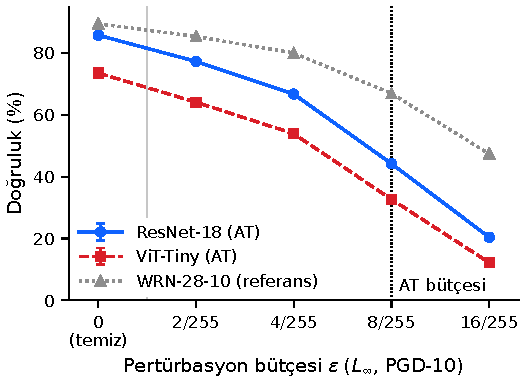
\includegraphics[width=\columnwidth]{../figures/final_tr/fig2_epsilon_sweep.pdf}
\caption{Pertürbasyon bütçesi $\eps$'a göre PGD-10 gürbüz doğruluğu, tam test kümesi (üç koşu ortalaması; $\pm$1 std hata çubukları işaretçilerden dardır). Yatay eksen kategoriktir ve $\eps=0$ temiz doğruluktur. Tarama ayrı bir PGD-10 değerlendirmesidir; bu yüzden $8/255$ noktası Tablo~\ref{tab:main_results}'den en çok $0{,}08$ puan ayrılır. CNN'in ViT üzerindeki marjı sabit değildir; küçük bütçelerde en geniş, $16/255$'te ise daralmış durumdadır.}
\label{fig:epsilon_sweep}
\end{figure}


% ----------------------------------------------------------------------------
% B. Protokoller ve ozdeslik
% ----------------------------------------------------------------------------
\subsection{Sabit Modeller Üzerinde Dört Koşullama Protokolü}
\label{subsec:transfer}

Her tohum çifti için PGD-10 çekişmeli örnekleri kaynak modelde üretilmiş ve tam test kümesinde bir hedef üzerinde değerlendirilmiştir. Sonuçlar örnek bazında kaydedildiğinden aynı saldırı koşusu, yeniden hesaplama gerekmeden Tablo~\ref{tab:protocol_masks}'teki her protokol altında puanlanabilmektedir; protokoller yalnızca paydaya hangi örneklerin girdiğinde ayrışmaktadır.

\begin{table}[!t]
\centering
\caption{Koşulsuz oran ve üç yerleşik koşullama protokolü altında transfer asimetrisi (PGD-10, $\eps$=8/255, tam test kümesi; üç tohum çifti üzerinden ortalama$\pm$std).}
\label{tab:transfer_protocols}
\footnotesize
\setlength{\tabcolsep}{3pt}
\begin{tabular}{lccc}
\toprule
\textbf{Protokol} & \textbf{CNN$\rightarrow$ViT} & \textbf{ViT$\rightarrow$CNN} & \textbf{Fark (puan)} \\
\midrule
Koşulsuz (ham) & 41,02$\pm$0,55 & 27,45$\pm$0,27 & $+$13,57$\pm$0,33 \\
Hedef doğru & 19,87$\pm$0,18 & 15,51$\pm$0,59 & $+$4,36$\pm$0,44 \\
Her ikisi doğru & 18,25$\pm$0,17 & 9,98$\pm$0,31 & $+$8,27$\pm$0,23 \\
Başarılı kaynak & 36,39$\pm$0,76 & 17,02$\pm$0,52 & $+$19,37$\pm$1,27 \\
\bottomrule
\end{tabular}
\end{table}

% Ic ice kosullama kumeleri sekli; TR surumu final_tr (surum 4: sag panelde uc ikili uzaklik).
\begin{figure}[!t]
\centering
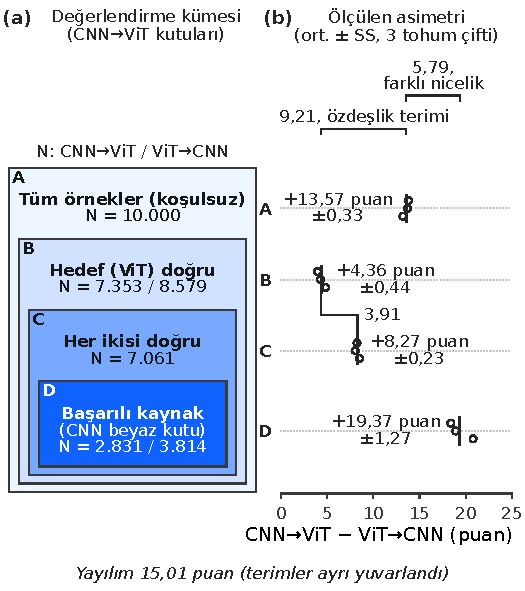
\includegraphics[width=\columnwidth]{../figures/final_tr/fig_protocol_sets.pdf}
\caption{Dört transfer protokolünün CNN$\rightarrow$ViT yönündeki iç içe değerlendirme kümeleri (a; kutular şematiktir ve alanla orantılı değildir, $N$ üç tohum çiftinin ortalamasıdır) ve her protokolün aynı modeller ve aynı veri üzerinde verdiği CNN$\rightarrow$ViT eksi ViT$\rightarrow$CNN asimetrisi (b; üç tohum çifti üzerinden çift içi eşleştirilmiş farkın ortalaması$\pm$SS, tek tek çiftler içi boş işaretçilerle). ViT$\rightarrow$CNN kümeleri aynı sırayla iç içedir ($N$ = 10.000, 8.579, 7.061 ve 3.814); koşulsuz ve her ikisi doğru kümeleri iki yönde aynıdır, diğer ikisi ise aynı değildir. (b) panelindeki bağlayıcılar üç ikili uzaklığı işaretlemektedir. CIFAR-10'da $15{,}01$ puanlık yayılım, başarılı kaynağın her ikisi doğru üzerindeki fazlası ($11{,}10$ puan, farklı bir nicelik) ile onaylanan ikili içindeki uzaklığın ($3{,}91$ puan) toplamıdır; koşulsuz kestirim bu aralığın içinde, Denklem~\eqref{eq:raw_identity}'in yerleştirdiği gibi hedef doğrunun $9{,}21$ puan üstünde yer almaktadır.}
\label{fig:protocol_sets}
\end{figure}

% REF: Tablo III: transfer protokolleri (N degerleri, 15.01 +- 0.84, ~4.4 kat)
% REF: Secim kuralinin asimetriye etkisi, B (kosumlar arasi araliklar 0.63 / 0.86 / 0.46 / 2.41)
Paydalar protokoller arasında keskin biçimde değişmektedir. CNN$\rightarrow$ViT ve ViT$\rightarrow$CNN için paydalar sırasıyla koşulsuz durumda 10.000/10.000, hedef doğruda 7.353/8.579, her ikisi doğruda 7.061 ortak örnek ve başarılı kaynakta 2.831/3.814'tür. Aynı modeller ve aynı veri üzerinde asimetri $+4{,}36\pm0{,}44$ ile $+19{,}37\pm1{,}27$ puan arasında değişmekte, uç değerler arasında 4,4 katlık bir oran bulunmakta ve en büyük ile en küçük protokol kestirimi arasındaki çift başına ortalama yayılım $15{,}01\pm0{,}84$ puan olmaktadır. Yeniden eğitim aynı niceliği çok daha az oynatmaktadır. Üç eğitim çifti boyunca asimetri, tablodaki sırayla dört protokol altında $0{,}63$, $0{,}86$, $0{,}46$ ve $2{,}41$ puanlık aralıklara yayılmaktadır; dolayısıyla benzeri benzeriyle, yani aralığı aralıkla karşılaştıran ölçüt $15{,}01$ puana karşı en çok $2{,}41$ puandır. Fark sütunundaki standart sapma ($0{,}23$ ile $1{,}27$ puan) çift içi eşleştirilmiş farka aittir ve iki yön çiftler boyunca birlikte değiştiği için yön başına yayılımlardan geri hesaplanamamaktadır.

% REF: Turetilmis, Protokol farklarinin farki (raw-tc +9.21+-0.76; ss-raw +5.79; ss-bc +11.10+-1.09; bc-tc +3.91+-0.32;
%      C100 raw-tc +13.58, bc-tc +5.97; L2 bc-tc +1.95; SVHN bc-tc +0.82 / +0.49)
% REF: Turetilmis, bc - tc kosum duzeyi %95 t araligi ([+3.12; +4.70]; C100 [+3.53; +8.40]; L2 [+1.33; +2.56])
Yayılım tek bir nicelik değildir. CIFAR-10'da yayılım bitişik protokoller arasındaki iki uzaklığa ayrılmaktadır (Şekil~\ref{fig:protocol_sets}b). Başarılı kaynak kestirimi kaynağın kendi beyaz kutu başarısızlığına koşullandığı için farklı bir niceliği, yani zaten işe yaramış bir saldırının ne ölçüde taşındığını kestirmektedir ve her ikisi doğru kestiriminin $11{,}10\pm1{,}09$ puan üstündedir. Yönlü iddialar için onaylanan ve yalnızca kaynağın da doğru olmasının gerekip gerekmediğiyle ayrışan iki protokol, hedef doğru ve her ikisi doğru, birbirinden $3{,}91\pm0{,}32$ puan uzaktadır; koşum düzeyindeki \%95 $t$ aralığı $[3{,}12;\ 4{,}70]$'tir (iki serbestlik derecesi). Bu uzaklık çözümleyicinin takdirinden değil iki farklı kestirilen nicelik arasındaki farktan doğmaktadır ve aşağıda betimlenen marjinal altkümeler onu açıklamaktadır. Her çiftte hedef doğru en küçük, başarılı kaynak en büyük kestirim olduğundan iki uzaklık birlikte $15{,}01$ puanlık aralığı oluşturmaktadır. Koşulsuz kestirim bu aralığın içinde, hedef doğrunun $9{,}21\pm0{,}76$ puan üstünde ve başarılı kaynağın $5{,}79$ puan altında yer almaktadır; hedeflerin temiz hataları, koşullu oranlar ve ölçülen öncül $p$ bilindiğinde Denklem~\eqref{eq:raw_identity} onu tam bu konuma yerleştirmektedir (Bölüm~\ref{subsubsec:matrix}). Onaylanan uzaklık CIFAR-100'de $5{,}97$ puan (aralık $[3{,}53;\ 8{,}40]$), $L_2$ bütçesi altında $1{,}95$ puan ($[1{,}33;\ 2{,}56]$), iki SVHN çiftinde ise $0{,}82$ ve $0{,}49$ puandır. CIFAR-100'de koşulsuz kestirim aralığın üst ucudur ve $13{,}58$ puanlık özdeşlik terimi $13{,}83$ puanlık yayılımın neredeyse tamamını oluşturmaktadır.

Protokol istatistiksel okumayı da değiştirmektedir. İki yönü aynı örnekler üzerinde puanlayan ve bu yüzden eşleştirilmiş çıkarımı destekleyen her ikisi doğru protokolünde fark $8{,}27\pm0{,}24$ puandır; bu değerin tablodaki $\pm0{,}23$'ten hafifçe ayrılmasının tek nedeni iki kestiricinin farklı olmasıdır. Her koşunun kendi eşleştirilmiş bootstrap güven aralığı vardır ($[7{,}61;\ 9{,}44]$, $[7{,}10;\ 9{,}01]$ ve $[7{,}28;\ 9{,}20]$). Uç noktaların ortalaması $[7{,}33;\ 9{,}22]$ aralığını vermektedir; bu aralık üç aralığın bir betimlemesidir ve kendi başına kapsama garantisi taşımamaktadır. Koşum düzeyinde çıkarım için koşumlar arası $t$ aralığı $[7{,}68;\ 8{,}86]$'dır. İşaret çevirme permütasyonunun $p$ değeri her tohumda $5\times10^{-5}$'in altındadır ve her aralık $\pm3$'ün tamamen dışında kaldığı için TOST üç marjın hiçbirinde ($\pm1$, $\pm2$ ve $\pm3$ puan) eşdeğerliği kuramamaktadır.

% REF: Turetilmis, Basarili-kaynak: siki ve gevsek okuma (+14.60; 10.45; +4.77+-0.39)
Protokol adları alt seçimleri de açık bırakmaktadır. Kaynağın temiz girdide zaten yanlış sınıflandırdığı örnekleri de içeri alan gevşek başarılı kaynak okumasında (Tablo~\ref{tab:protocol_masks}) ölçülen asimetri $+19{,}37$ puandan $+14{,}60$ puana, protokol yayılımı ise $15{,}01$ puandan $10{,}45$ puana inmektedir. Bu $4{,}77\pm0{,}39$ puanlık kayma, Tablo~\ref{tab:transfer_protocols}'teki herhangi bir protokolün koşumlar arası standart sapmasından üç kattan fazla büyüktür; diğer üç protokol ise yapısı gereği değişmemektedir.

CIFAR-10'da kararlı olan yöndür. CNN'de üretilen örnekler ViT'e, dört protokolün dördünde, üç tohumun üçünde ve momentum tabanlı MI-FGSM~\cite{dong2018boosting} altında da tersinden daha iyi transfer olmaktadır ($19{,}07\pm0{,}33$'e karşı $\%15{,}42\pm0{,}52$, hedef doğru; bu iki yönlü kontrol başka yerde kullanılan $\alpha=2/255$ yerine saldırının kendi varsayılan adımı olan $\alpha=\eps/10$'u kullanmaktadır ve ViT$\rightarrow$CNN değerinin Tablo~\ref{tab:tgr}'deki eşleşmiş bütçeli değerden hafifçe ayrılmasının nedeni budur). Dolayısıyla etki PGD saldırısının kendisinin bir artefaktı değildir. Etkinin büyüklüğü ve anlamlılığı, onlarla birlikte de her türlü eşdeğerlik iddiası protokole bağlıdır.

Onaylanan iki protokol arasındaki uzaklığın bileşimsel bir kaynağı vardır. Hedefin temizde çözdüğü ama kaynağın çözemediği örnekler ortak çözülenlerden üç-dört kat daha kırılgandır ($\%41{,}2\pm0{,}8$ ve $\%59{,}1\pm1{,}7$ yanıltmaya karşı $\%10{,}0$ ve $\%18{,}2$) ve bu marjinal altkümeler, iki model temiz doğrulukta ayrıştığı için boyutça beş kat farklıdır ($1.517\pm102$'ye karşı $291\pm16$). Hedef doğru koşullaması iki marjinal altkümeyi de içeri almakta ve bunların asimetrik boyutları iki oranı birbirine doğru çekmektedir; her ikisi doğru koşullaması ise onları dışarıda bırakmakta ve yönlü fark yeniden ortaya çıkmaktadır. Bu açıklama dört protokolün üçünü kapsamaktadır. Başarılı kaynak protokolü \emph{kaynağın} kendi gürbüzlüğüne göre seçim yapmaktadır; bu gürbüzlük çiftin temiz doğruluk farkının bir fonksiyonu olmadığından protokol ikinci, kısmen ters yönlü bir terim katmaktadır (Bölüm~\ref{subsubsec:spread_gap}).

% ----------------------------------------------------------------------------
% B.1 Uc mimarili kontrol ve oncul p
% ----------------------------------------------------------------------------
\subsubsection{Ham oranın ne kadarı hedefin temiz hatası?}
\label{subsubsec:matrix}

% REF: C3: WRN dahil 3x3 matris (r = 0.997; egim 0.762)
% REF: Dis veri: Mahmood, "Ozdeslikte kullanilan p" (p_min 0.989014, results/q1/ozdeslik_kontrol.json)
WideResNet-28-10 referansının hem kaynak hem hedef olarak eklenmesi her eğitim çifti için bir $3\times3$ matris vermektedir (Tablo~\ref{tab:transfer_matrix}); Denklem~\eqref{eq:raw_identity} bu matrisin altı köşegen dışı yönünde, temiz hataları birbirinden çok farklı hedeflere karşı sınanabilmektedir. Özdeşliğin öncülü bu çekişmeli eğitilmiş hedeflerde sıkı biçimde sağlanmaktadır. $36$ köşegen dışı yönde (iki veri kümesi, üç tohum çifti, üç hedef, iki kaynak) ölçülen $p$ değeri $0{,}989$ ile $1{,}000$ arasındadır. Bu nedenle $p=1$ biçimi ölçülen her koşulsuz oranı $0{,}41$ puan içinde yeniden üretmektedir; ortalama mutlak artık $0{,}095$ puandır ve artık, açıkladığı sapmanın en çok $\%1{,}39$'u kadardır. Bu artık puan cinsinden yeniden yazılmış öncül, yani $e\,(1-p)$ olduğundan ikinci bir doğrulama sayılmamaktadır; bilgi taşıyan nicelik $p$'nin kendisidir. Aynı sonuç sapma ile hedefin temiz hatası arasındaki bir korelasyon olarak ifade edilseydi ($r = 0{,}997$) eksik anlatılmış olurdu, çünkü bir niceliğin kendi baskın bileşeniyle bire yakın korelasyonu aritmetiktir.

Veri kümesine özgü kalan şey orantı çarpanıdır. $(1 - r_{\text{koş}})$ saldırının ne kadar transfer edilebilir olduğuna bağlı olduğundan uydurulan eğim CIFAR-10'da hedef hatasının puanı başına $0{,}762$, CIFAR-100'de $0{,}656$ puandır. Bu eğim ölçülen hedefler üzerinden bir ortalamadır ve özdeşlik başka model havuzlarına her uygulandığında yeniden kestirilmelidir. Koşulsuz transfer oranları bu yüzden mimariler arası transfer edilebilirliği ölçmemekte, transfer edilebilirliği hedefin temiz zayıflığıyla birlikte, Denklem~\eqref{eq:raw_identity}'in açıkça gösterdiği bir oranda ölçmektedir.

\begin{table}[!t]
\centering
\caption{$3\times3$ transfer matrisi (PGD-10, $\eps$=8/255, tam test kümesi; üç tohum çifti üzerinden ortalama$\pm$std; WideResNet satır ve sütunu tek harici kontrol noktasını kullanır). Ham = koşulsuz yanıltma oranı, Koş. = hedef doğru koşullu oran. Köşegen girdileri beyaz kutu saldırılardır. Bu matrisin saldırıları ayrı bir koşuda üretilmiştir (saldırı tohumu 42); Tablo~\ref{tab:conditional} ve Tablo~\ref{tab:transfer_protocols} ile paylaştığı hücreler onlardan en çok $0{,}06$ puan ayrılır ve bu fark Bölüm~\ref{subsec:statistics_results}'teki saldırı başlatma varyansının içindedir.}
\label{tab:transfer_matrix}
\footnotesize
\setlength{\tabcolsep}{3pt}
\begin{tabular}{llcc}
\toprule
\textbf{Kaynak} & \textbf{Hedef} & \textbf{Ham (\%)} & \textbf{Koş.\ (\%)} \\
\midrule
ResNet-18 AT & ResNet-18 AT & 55,84$\pm$0,53 & 48,52$\pm$0,84 \\
ResNet-18 AT & ViT-Tiny AT & 41,07$\pm$0,58 & 19,93$\pm$0,20 \\
ResNet-18 AT & WRN-28-10 & 21,69$\pm$0,09 & 12,48$\pm$0,10 \\
ViT-Tiny AT & ResNet-18 AT & 27,45$\pm$0,34 & 15,52$\pm$0,64 \\
ViT-Tiny AT & ViT-Tiny AT & 67,34$\pm$0,18 & 55,57$\pm$0,44 \\
ViT-Tiny AT & WRN-28-10 & 18,25$\pm$0,12 & 8,65$\pm$0,14 \\
WRN-28-10 & ResNet-18 AT & 32,63$\pm$0,14 & 21,48$\pm$0,31 \\
WRN-28-10 & ViT-Tiny AT & 39,73$\pm$0,25 & 18,15$\pm$0,28 \\
WRN-28-10 & WRN-28-10 & 33,03 & 25,16 \\
\bottomrule
\end{tabular}
\end{table}

% ----------------------------------------------------------------------------
% C. Kaynak etkisi
% ----------------------------------------------------------------------------
\subsection{Hedef Zayıflığı Değil, Kaynak Etkisi}
\label{subsec:source_target}

Üç mimarili $3\times3$ matrisler yönün nereden geldiğini de göstermektedir. Bir CNN$\rightarrow$ViT üstünlüğü, CNN'de üretilen örneklerin herhangi bir hedefe daha iyi taşınmasından, yani bir kaynak etkisinden ya da ViT'in herhangi bir kaynak için daha kolay hedef olmasından, yani bir hedef etkisinden doğabilir. İki etki, her eğitim çiftinin altı köşegen dışı oranına protokol protokol uydurulan ve toplamı sıfır kodlama kullanan $r(s\rightarrow t) = \mu + \alpha_s + \beta_t + \varepsilon_{st}$ toplamsal modeliyle ayrılmıştır. Böylece asimetri, kaynak farkı $\alpha_{\text{CNN}} - \alpha_{\text{ViT}}$, hedef farkı $\beta_{\text{ViT}} - \beta_{\text{CNN}}$ ve bir artık farkının toplamına eşit olmaktadır. Altı hücre ve beş parametre tek bir artık serbestlik derecesi bıraktığından yüksek bir $R^2$ beklenen bir sonuçtur ve az kanıt taşımaktadır; uydurma her matrisi betimlemekte, hiçbir şeyi sınamamaktadır, aşağıdaki sabit üçüncü model karşıtlıkları ise hiçbir model gerektirmemektedir.

% REF: Kaynak-hedef toplamsal ayristirma, CIFAR-10 ve CIFAR-100 cift basina ayristirma (tc, bc, ss, ham)
% REF: Kaynak-hedef toplamsal ayristirma, sabit-WRN karsitliklari; C3: WRN dahil 3x3 matris (gelen transfer; r = 0.986)
Kaynak terimi asimetriyi iki veri kümesinde de taşımaktadır (Tablo~\ref{tab:source_target}). CIFAR-10'da kaynak farkı $+5{,}13\pm0{,}09$, hedef farkı $-2{,}03\pm0{,}51$ puandır. ViT üzerinde üretilen örnekler daha kötü taşınmakta ve ViT iki hedefin \emph{daha az} kırılgan olanı olmaktadır; dolayısıyla hedef terimi ölçülen $+4{,}41\pm0{,}45$ puanlık asimetriye karşı çalışmaktadır. CIFAR-100 aynı örüntüyü daha büyük ölçekte yinelemektedir ($+9{,}54\pm0{,}64$'e karşı $-6{,}19\pm0{,}93$). Kaynak terimi puanlanabilen her protokolde işaretini korurken hedef terimi korumamaktadır. Her ikisi doğru protokolünde hedef farkı CIFAR-10'da sıfırdan ayırt edilemeyen $-0{,}53\pm0{,}59$, CIFAR-100'de $-2{,}85\pm0{,}93$ olurken kaynak farkı $+6{,}76\pm0{,}35$ ve $+11{,}79\pm0{,}83$'e çıkmaktadır; CIFAR-100 kayıtlarının izin verdiği başarılı kaynak protokolünde ise terimler $+20{,}82\pm1{,}43$ ve $-8{,}12\pm2{,}23$'tür. WideResNet aynı karşıtlıkları model gerektirmeden sağlamaktadır. Sabit bir hedef olarak WideResNet, ResNet'te üretilen örneklerin $\%12{,}48$'i, ViT'te üretilenlerin ise $\%8{,}65$'i ile kandırılmaktadır; yani ViT'te üretilen örnekler üçüncü bir mimariye bile daha kötü taşınmaktadır. Sabit bir kaynak olarak ise ResNet'i $\%21{,}48$, ViT'i $\%18{,}15$ oranında kandırmaktadır; dolayısıyla ViT üçüncü bir modelin pertürbasyonları için de daha zor hedeftir. Sabit model karşıtlıkları her ikisi doğru protokolünde de bu işaretleri korumakta (CIFAR-10'da $+4{,}69\pm0{,}38$ ve $-2{,}60\pm0{,}72$), hedef karşıtlığı ise iki veri kümesinde de her koşullu protokolde negatif kalmaktadır. Ham oranlarla puanlandığında aynı ayrıştırma CIFAR-10'da $+8{,}13$, CIFAR-100'de $+10{,}72$ puanlık bir hedef farkı vermektedir; koşulsuz oranlar ViT'in daha büyük temiz hatasını da saydığı için onu daha zayıf hedef gibi göstermektedir. Daha zayıf hedef okuması gelen transfer korelasyonuna da dayandırılamaz. Gelen koşullu transfer her hedefin kendi beyaz kutu koşullu yanıltma oranını izlemektedir (üç hedef üzerinde $r = 0{,}986$), ancak bu korelasyonu iki aileden gelen saldırıları da soğuran gürbüz WideResNet taşımaktadır ($\%10{,}57$ gelen transfer). ResNet ile ViT arasında gelen transfer yalnızca $0{,}54$ puan farklıdır ($\%18{,}50$'ye karşı $\%19{,}04$), asimetri ise $4{,}41$ puandır.

% REF: Kaynak-hedef toplamsal ayristirma, Mahmood ve ark. (2021) CIFAR-10 ve CIFAR-100 8x8 uydurmalari
% REF: Dis veri: Mahmood ve ark., Aile duzeyi asimetri ve guclu kaynak ailesi sayimi (12/12; 6/6)
Mahmood vd.'nin~\cite{mahmood2021robustness} $8\times8$ matrisleri, başka yerde eğitilmiş modeller üzerinde aynı ayrıştırmaya imkân vermektedir. Bu matrisler kendi her ikisi doğru protokolleri altında, çift başına $m=1000$ örnekle ve her hücrede FGSM, PGD ve MIM saldırılarının en güçlüsüyle ($\eps=0{,}031$) elde edilmiştir. Mahmood vd.'nin rejimi bu karşılaştırma için önemli olan her bakımdan buradakinden farklıdır. ViT ve BiT-M modelleri ImageNet-21k üzerinde ön eğitilmiş ve çekişmeli eğitim olmadan ince ayarlanmış, ResNet-56 ve ResNet-164 ise CIFAR üzerinde çekişmeli eğitim olmadan eğitilmiştir; köşegenleri de beyaz kutu saldırısı değil aynı modelin bağımsız eğitilmiş bir kopyası olduğundan dışarıda bırakılmıştır. Aile içi transfer aileler arası transferden çok daha güçlü olduğu için toplamsal model bu matrislere zayıf uymaktadır (CIFAR-10'da $R^2=0{,}368$, CIFAR-100'de $0{,}451$); aynı aile terimi $R^2$'yi $0{,}785$ ve $0{,}843$'e çıkarmaktadır. İki uydurmada da aile düzeyindeki kaynak farkı CIFAR-10'da ViT lehinedir (CNN eksi ViT olarak toplamsal uydurmada $-25{,}01$, aile terimiyle $-10{,}78$ puan) ve buradaki yönün tersini göstermektedir; melez ViT-R50'nin dışarıda bırakıldığı $12$ aileler arası çiftin tamamında da ViT daha güçlü kaynaktır. CIFAR-100'de ResNet-56 ve ResNet-164 bu çalışmanın yönünü göstermekte ve $6/6$ çiftte CNN$\rightarrow$ViT daha güçlü olmaktadır; ancak bu yönü hedef terimi taşımakta (toplamsal $+30{,}15$, aile terimiyle $+16{,}81$), kaynak terimi ise yine ViT lehine kalmaktadır ($-21{,}90$ ve $-8{,}55$). Orada yön buradakiyle uyuşmakta, mekanizma ise uyuşmamaktadır. Bölüm~\ref{subsec:findings} bu durumun açık bıraktığı soruyu tartışmaktadır.

% REF: tablo hucrelerinin tamami "Kaynak-hedef toplamsal ayristirma" ve "Dis veri: Mahmood ve ark." bolumlerinden.
\begin{table*}[!t]
\centering
\caption{Transfer matrislerinin toplamsal kaynak-hedef ayrıştırması (puan; köşegen dışı hücreler). Kaynak farkı $=\alpha_{\text{CNN}}-\alpha_{\text{ViT}}$ (pozitif değer CNN'de üretilen örneklerin daha iyi taşındığını gösterir); hedef farkı $=\beta_{\text{ViT}}-\beta_{\text{CNN}}$ (pozitif değer ViT'in daha kırılgan hedef olduğunu gösterir); asimetri $=$ CNN$\rightarrow$ViT eksi ViT$\rightarrow$CNN. Üst blok: bu çalışmanın $3\times3$ matrisleri (ResNet-18 AT, ViT-Tiny AT, WideResNet-28-10; standart eğitilmiş satırda her çiftin temiz eğitilmiş ResNet-18 ve ViT-Tiny modelleri ile RobustBench'in standart WideResNet-28-10 modeli), eğitim çifti ve protokol başına uydurulmuş, üç çift üzerinden ortalama$\pm$std. Matrisler Tablo~\ref{tab:transfer_matrix}'deki ayrı saldırı koşusundan geldiği için CIFAR-10 hedef doğru asimetrisi burada $4{,}41$, Tablo~\ref{tab:transfer_protocols}'te $4{,}36$'dır; altı hücre ve beş parametreyle $R^2$ sınamaz, yalnızca betimler. Orta blok: uydurma yapılmadan sabit üçüncü model olarak WideResNet; hedef olarak bir kaynak karşıtlığı (CNN'den gelen oran eksi ViT'ten gelen oran), kaynak olarak bir hedef karşıtlığı (ViT'e giden oran eksi CNN'e giden oran) verir. Alt blok: Mahmood vd.'nin~\cite{mahmood2021robustness} $8\times8$ her ikisi doğru matrisleri (standart eğitilmiş modeller, $m$=1000, köşegen hariç); aksi belirtilmedikçe melez ViT-R50 dışındaki CNN ve ViT aileleri, aynı aile terimli ve terimsiz uydurmalar.}
\label{tab:source_target}
\footnotesize
\setlength{\tabcolsep}{4pt}
\begin{tabular}{llccccc}
\toprule
\textbf{Veri} & \textbf{Protokol ya da uydurma} & \textbf{Kaynak farkı} & \textbf{Hedef farkı} & \textbf{Asimetri} & \textbf{En büyük $|$artık$|$} & \textbf{$R^2$} \\
\midrule
\multicolumn{7}{l}{\textit{Bu çalışmanın matrisleri, eğitim çifti başına toplamsal uydurma}} \\
CIFAR-10 & Hedef doğru & $+$5,13$\pm$0,09 & $-$2,03$\pm$0,51 & $+$4,41$\pm$0,45 & 0,65$\pm$0,05 & 0,9782$\pm$0,0032 \\
CIFAR-10 & Her ikisi doğru & $+$6,76$\pm$0,35 & $-$0,53$\pm$0,59 & $+$8,30$\pm$0,16 & 1,04$\pm$0,11 & 0,9643$\pm$0,0072 \\
CIFAR-10 & Koşulsuz & $+$4,47$\pm$0,10 & $+$8,13$\pm$0,33 & $+$13,62$\pm$0,38 & 0,51$\pm$0,03 & 0,9964$\pm$0,0004 \\
CIFAR-100 & Hedef doğru & $+$9,54$\pm$0,64 & $-$6,19$\pm$0,93 & $+$4,96$\pm$1,02 & 0,80$\pm$0,05 & 0,9871$\pm$0,0015 \\
CIFAR-100 & Her ikisi doğru & $+$11,79$\pm$0,83 & $-$2,85$\pm$0,93 & $+$10,92$\pm$0,34 & 0,99$\pm$0,10 & 0,9851$\pm$0,0035 \\
CIFAR-100 & Başarılı kaynak & $+$20,82$\pm$1,43 & $-$8,12$\pm$2,23 & $+$17,50$\pm$0,92 & 2,40$\pm$0,06 & 0,9830$\pm$0,0008 \\
CIFAR-100 & Koşulsuz & $+$6,48$\pm$0,38 & $+$10,72$\pm$0,97 & $+$18,53$\pm$0,71 & 0,67$\pm$0,01 & 0,9946$\pm$0,0003 \\
C10, standart eğitim & Hedef doğru & $+$69,18$\pm$2,31 & $-$75,05$\pm$1,72 & $-$4,49$\pm$0,85 & 0,69$\pm$0,20 & 0,9996$\pm$0,0002 \\
\midrule
\multicolumn{7}{l}{\textit{Sabit üçüncü model olarak WideResNet-28-10, uydurma yok}} \\
CIFAR-10 & Hedef doğru & $+$3,83$\pm$0,17 & $-$3,33$\pm$0,59 & -- & -- & -- \\
CIFAR-10 & Her ikisi doğru & $+$4,69$\pm$0,38 & $-$2,60$\pm$0,72 & -- & -- & -- \\
CIFAR-100 & Hedef doğru & $+$7,94$\pm$0,54 & $-$7,79$\pm$0,95 & -- & -- & -- \\
CIFAR-100 & Her ikisi doğru & $+$9,81$\pm$1,03 & $-$4,83$\pm$0,75 & -- & -- & -- \\
CIFAR-100 & Başarılı kaynak & $+$16,03$\pm$1,42 & $-$12,91$\pm$2,29 & -- & -- & -- \\
C10, standart eğitim & Hedef doğru & $+$67,80$\pm$2,11 & $-$76,43$\pm$2,02 & -- & -- & -- \\
\midrule
\multicolumn{7}{l}{\textit{Mahmood vd.~\cite{mahmood2021robustness}, $8\times8$ her ikisi doğru matrisler, aile düzeyi}} \\
CIFAR-10 & Toplamsal & $-$25,01 & $+$2,08 & $-$24,01 & 74,04 & 0,3681 \\
CIFAR-10 & Aynı aile terimi & $-$10,78 & $-$12,15 & $-$24,01 & 29,33 & 0,7852 \\
CIFAR-100 & Toplamsal & $-$22,77 & $+$14,74 & $-$9,02 & 66,29 & 0,4508 \\
CIFAR-100 & Aynı aile terimi & $-$9,43 & $+$1,39 & $-$9,02 & 24,33 & 0,8425 \\
CIFAR-100 & ResNet-56/164 ile ViT, toplamsal & $-$21,90 & $+$30,15 & $+$9,15 & -- & -- \\
CIFAR-100 & ResNet-56/164 ile ViT, aynı aile & $-$8,55 & $+$16,81 & $+$9,15 & -- & -- \\
\bottomrule
\end{tabular}
\end{table*}

% ----------------------------------------------------------------------------
% D. Ayarlar arasi
% ----------------------------------------------------------------------------
\subsection{Veri Kümeleri ve Tehdit Modelleri Arasında}
\label{subsec:settings}

Tablo~\ref{tab:protocol_settings} bu makaledeki her ayarda dört protokolü bir araya getirmektedir. Onaylanan iki protokol her ayarın içinde aynı işareti vermektedir; protokoller arasında işaret yalnızca SVHN'de değişmekte ve orada dört kestirimin tamamı sıfırın üç puan yakınında kalmaktadır. Ayarlar aşağıda sırayla ele alınmakta (Bölüm~\ref{subsec:cifar100} ile~\ref{subsec:l2} arası), ardından ölçülen her çiftte yayılım ile temiz doğruluk farkı arasındaki ilişki incelenmektedir (Bölüm~\ref{subsubsec:spread_gap}).

% ----------------------------------------------------------------------------
% D.1 Ikinci veri kumesi (E1)
% ----------------------------------------------------------------------------
\subsubsection{İkinci bir veri kümesi: CIFAR-100}
\label{subsec:cifar100}

Yalnızca CIFAR-10'da var olan bir protokol etkisi genel bir raporlama önerisini desteklemeyeceği için tasarımın tamamı CIFAR-100 üzerinde yinelenmiştir; mimariler, tehdit modeli, saldırı bütçesi, üç tohumlu yapı ve dört protokol aynı tutulmuştur. Üç yönsel ön kestirim ile üç uç nokta bandı, bu veri kümesinden herhangi bir ölçüm mevcut olmadan önce salt eklemeli bir belgeye kaydedilmiş, böylece sonucun ölçüldükten sonra yeniden yorumlanmasının önüne geçilmiştir. Kayıt eğitimin başlangıcından önce gelmemektedir; kayıt işlemesi, sayı bildiren ilk adımdan, yani epok 5'teki pilot kapısından altmış altı dakika öncedir.

\begin{table}[!t]
\centering
\caption{CIFAR-100 yinelemesi (mimari başına üç bağımsız eğitim koşusunun ortalaması$\pm$std, tam test kümesi, $\eps$=8/255). İki model de Bölüm~\ref{subsec:training}'deki tarifle eğitilmiştir. Mutlak gürbüzlük iki mimaride de CIFAR-10'a göre düşüktür ve CNN'in ViT üzerindeki sıralaması değişmemiştir.}
\label{tab:cifar100_results}
\footnotesize
\begin{tabular}{lccc}
\toprule
\textbf{Model} & \textbf{Temiz (\%)} & \textbf{PGD-10 (\%)} & \textbf{AutoAttack (\%)} \\
\midrule
ResNet-18 AT & 63,86$\pm$1,05 & 19,30$\pm$0,32 & 15,04$\pm$0,54 \\
ViT-Tiny AT  & 43,17$\pm$1,10 & 11,15$\pm$0,60 & 8,87$\pm$0,83 \\
\bottomrule
\end{tabular}
\end{table}

Mutlak gürbüzlük CIFAR-10'a göre düşüktür ve CNN'in ViT üzerindeki sıralamasını korumaktadır (Tablo~\ref{tab:cifar100_results}). Aynı dört protokol boyunca ölçülen CNN$\rightarrow$ViT asimetrisi $+4{,}96\pm1{,}01$ puandan (hedef doğru) $+18{,}53\pm0{,}71$ puana (koşulsuz) uzanmakta; her ikisi doğru protokolünde $+10{,}92\pm0{,}34$, başarılı kaynak protokolünde ise $+17{,}50\pm0{,}92$ puan olmaktadır. Tohum başına ortalama yayılım $13{,}83\pm1{,}30$ puandır; CIFAR-10'da bu değer $15{,}01\pm0{,}84$ olduğuna göre daha zor veri kümesi protokol etkisini aynı aralıkta, CIFAR-10 değerinin bir miktar altında bırakmaktadır. Yön, CIFAR-10'da olduğu gibi on iki ölçümün tamamında pozitiftir (dört protokol $\times$ üç tohum çifti). Her ikisi doğru protokolünde eşleştirilmiş fark $10{,}92$ puandır. CIFAR-10'da olduğu gibi verilen $[9{,}47;\ 12{,}35]$ aralığı üç tohumun kendi bootstrap uç noktalarının ortalamasıdır ve kapsama garantisi taşımamaktadır; mimarilere ilişkin bir iddiayla eşleşen koşumlar arası $t$ aralığı ise $[10{,}07;\ 11{,}77]$'dir. İşaret çevirme permütasyonunun $p$ değeri her tohumda $20.000$ permütasyonun çözünürlüğünün altındadır ve TOST sınanan hiçbir marjda eşdeğerliği kuramamaktadır.

Kaydedilen üç ön kestirimin biri doğrulanmış, biri bağlayıcı kabul edilen okumada tutmamış, üçüncüsü ise bu tasarımda sınanamamıştır. İşaretin korunacağı ön kestirimi doğrulanmıştır ($12/12$). Protokol yayılımının daha zor veri kümesinde büyüyeceği ön kestirimi CIFAR-10 yayılımına karşı bir karşılaştırma olarak kaydedilmiş ve o tarihte bu yayılım $10{,}45$ puan olarak anılmıştı. Bu sayısal eşiğe karşı kestirim tutmaktadır ($13{,}83 > 10{,}45$); sıkı başarılı kaynak okuması altındaki güncel CIFAR-10 yayılımına karşı ise tutmamaktadır ($13{,}83 < 15{,}01$). Kayıt sayıyı değil CIFAR-10 yayılımını adlandırdığı için bu sonuç bir başarısızlık olarak sayılmıştır. Üçüncü ön kestirim, koşulsuz oranın koşullu orandan sapmasının hedefin temiz hatasıyla birlikte büyüyeceğini öngörüyordu. Ölçülen eğim hedef hatasının puanı başına $+0{,}656$ puandır ve öngörüldüğü gibi pozitiftir. Ancak CIFAR-100'de üç hedeften ikisinin temiz hatası yalnızca $0{,}21$ puan farklıdır ($36{,}15$ ve $36{,}36$); dolayısıyla korelasyon üç değil iki etkin küme üzerinden hesaplanmakta ve değeri (altı yön üzerinde $r = 0{,}931$, hedef düzeyinde $0{,}974$) iki noktalı bir karşıtlığa dayanmaktadır. Ölçüm ön kestirimi \emph{sınamadan} onunla \emph{tutarlıdır} ve üçüncü bir doğrulama sayılmamaktadır.

Kaydedilen uç noktalardan biri tutmamıştır. Çekişmeli eğitilmiş ViT için temiz doğruluk $\%33$ ile $40$ bandında öngörülmüş, $\%43{,}17\pm1{,}10$ ölçülmüştür. Bant, çekişmeli eğitimin temiz doğruluk bedelinin iki mimaride aynı biçimde ölçekleneceği varsayımıyla türetilmişti. Bu varsayım tutmamıştır; ViT çekişmeli eğitim altında temiz ön eğitim doğruluğunun $0{,}885$'ini korurken ResNet $0{,}802$'sini korumuştur. Protokol iddiasının dayandığı iki çekişmeli uç nokta ise bantlarının içinde kalmıştır (PGD-10 öngörüsü $\%10$ ile $14$, ölçüm $11{,}15$; AutoAttack öngörüsü $\%8$ ile $11$, ölçüm $8{,}87$). Koşullama sınıf karışımını da değiştirdiğinden bir asimetri ilke olarak bir bileşim artefaktı olabilirdi, ancak ölçümler bunu göstermemektedir. Hedef doğru protokolünde asimetrinin bileşim bileşeni üç tohum çiftinde $-1{,}249$, $-1{,}330$ ve $-1{,}065$ puandır ve \emph{negatiftir}; yani sınıf karışımı yeniden dengelenseydi asimetri büyürdü. Başarılı kaynak protokolünde bu bileşen küçüktür ve her tohumda pozitiftir ($+0{,}527$, $+0{,}435$ ve $+0{,}382$ puan); koşulsuz ve her ikisi doğru protokollerinde ise ayrıştırmanın gerektirdiği gibi tam olarak sıfırdır.

Bu sonuç iki niteleme taşımaktadır. Birincisi, iki çekişmeli bant en yakın tohum düzeyi kenarında $0{,}22$ puanlık (AutoAttack) ve $0{,}48$ puanlık (PGD-10) marjlarla tutmuştur ve bu marjlar aynı veri kümesindeki kontrol noktası seçimi gürültüsünden küçüktür. Eğitim koşusu sabit tutularak CIFAR-100 yörüngelerinde erken durdurma sabrı ve eğri yumuşatması tarandığında raporlanan PGD-10 doğruluğu $0{,}18$ ile $1{,}83$ puan arasında oynamaktadır (ortalama $0{,}86$). Aynı dokuz hücreli tarama CIFAR-10'da doğrulama bölmesi başına $0{,}54$ ile $2{,}83$ puan vermektedir; Bölüm~\ref{subsec:selection}'deki on sekiz hücreli değer ise bölmeyi de değiştirdiği için daha da büyüktür ve CIFAR-100 protokolünde bu boyut bulunmamaktadır. İkincisi, iki bağımsız bölme yerine aynı ayrılmış bölme iki aşamada da seçim için kullanılmıştır; bu tercih iki veri kümesini karşılaştırılabilir tutmak amacıyla CIFAR-10 protokolünden devralınmıştır.

% ----------------------------------------------------------------------------
% D.2 Ucuncu veri kumesi: SVHN, esleşmeye yakin cift
% ----------------------------------------------------------------------------
\subsubsection{Eşlenmeye yakın bir çiftle üçüncü bir veri kümesi: SVHN}
\label{subsec:svhn}

CIFAR-10 ve CIFAR-100 iki mimariyi temiz doğrulukta birbirinden hayli uzağa yerleştirmektedir (yaklaşık $12$ ve $21$ puan). SVHN~\cite{netzer2011reading} ise böyle değildir. Aynı tarifle çekişmeli eğitildiğinde ResNet iki koşuda $\%94{,}76$ ve $\%93{,}77$ (ortalama $94{,}27$), ViT ise $\%92{,}82$ ve $\%92{,}03$ (ortalama $92{,}42$) temiz doğruluğa ulaşmakta, aradaki farklar $1{,}94$ ve $1{,}74$ puan (ortalama $1{,}84$) olmaktadır. İki koşudan hesaplanan $0{,}70$ ve $0{,}56$'lık standart sapmalar az bilgi taşıdığından koşu değerleri ayrı ayrı verilmiştir. Ortalama gürbüz doğruluklar PGD-10 altında $\%55{,}52$ ve $\%52{,}30$'dur. PGD-10 farkı hâlâ yaklaşık üç puan olduğundan bu çift eşlenmiş değil, eşlenmeye yakın olarak adlandırılmaktadır. Özdeşlik terimi temiz doğruluk farkını izliyorsa burada yönün kendisi bir protokol meselesine dönüşmelidir.

\begin{table*}[!t]
\centering
\caption{Bu makaledeki her ayarda dört koşullama protokolü altında transfer asimetrisi (CNN$\rightarrow$ViT eksi ViT$\rightarrow$CNN, yüzde puan; PGD-10; $L_\infty$ altında $\eps$=8/255, $L_2$ altında $\eps$=0,5; tam test kümeleri). Üç tohum çiftli ayarlarda çiftler üzerinden ortalama$\pm$std verilir; SVHN'de iki çift olduğundan standart sapma yerine iki değer ayrı ayrı basılır. Yayılım, çift başına dört protokol üzerindeki açıklığın çiftler üzerinden ortalamasıdır. Onaylanan iki protokol, hedef doğru ve her ikisi doğru, her ayarın içinde aynı işareti verir; protokoller arasında işaret yalnızca SVHN'de değişir ve orada dört kestirimin tamamı sıfırın üç puan yakınındadır.}
\label{tab:protocol_settings}
\footnotesize
\begin{tabular}{lcccc}
\toprule
\textbf{Protokol} & \textbf{CIFAR-10, $L_\infty$} & \textbf{CIFAR-100, $L_\infty$} & \textbf{SVHN, $L_\infty$} & \textbf{CIFAR-10, $L_2$} \\
 & 3 çift, $n$=10.000 & 3 çift, $n$=10.000 & 2 çift, $n$=26.032 & 3 çift, $n$=10.000 \\
\midrule
Koşulsuz (ham) & $+$13,57$\pm$0,33 & $+$18,53$\pm$0,71 & $+$0,33 / $+$0,45 & $+$13,03$\pm$0,81 \\
Hedef doğru & $+$4,36$\pm$0,44 & $+$4,96$\pm$1,01 & $-$1,16 / $-$0,85 & $+$2,12$\pm$0,18 \\
Her ikisi doğru & $+$8,27$\pm$0,23 & $+$10,92$\pm$0,34 & $-$0,34 / $-$0,36 & $+$4,07$\pm$0,36 \\
Başarılı kaynak & $+$19,37$\pm$1,27 & $+$17,50$\pm$0,92 & $+$2,98 / $+$2,41 & $+$12,06$\pm$0,23 \\
\midrule
Yayılım (en büyük $-$ en küçük) & 15,01$\pm$0,84 & 13,83$\pm$1,30 & 4,14 / 3,26 & 10,92$\pm$0,82 \\
\bottomrule
\end{tabular}
\end{table*}

% REF: Transfer asimetrisi, dort protokol, ayarlar (SVHN satirlari; Her ikisi dogru, eslesmis analiz: SVHN)
Ölçümler bu beklentiyle uyuşmaktadır. Dört protokolün ikisi CNN, ikisi ViT üstünlüğü bildirmektedir (Tablo~\ref{tab:protocol_settings}). Yönlü iddialar için onaylanan iki protokol, hedef doğru ile her ikisi doğru, birbiriyle uyuşmakta ve ikisi de ViT lehine çıkmaktadır; işaret değişimi bu iki protokolü koşulsuz ve başarılı kaynak oranlarından ayırmaktadır. Koşulsuz orandaki çevrilme Denklem~\eqref{eq:raw_identity}'den aritmetik olarak çıkmaktadır. Burada ViT hedefinin temiz hatası CNN'inkini yaklaşık iki puan aşmakta ve bu fark $-1{,}00$'lık hedef doğru farkını $+0{,}39$'luk ham farka taşımaya yetmektedir. İki yönü özdeş örnekler üzerinde puanladığı için birincil kabul edilen her ikisi doğru protokolünde fark $-0{,}35$ puandır; işaret çevirme permütasyonunun $p$ değeri $0{,}105$'tir ve TOST eşdeğerliği, sınanan en dar marj ($\pm1$ puan) dahil üç marjın üçünde de kabul edilmektedir. Böyle bir eşdeğerlik iddiasının kurulup kurulamayacağına da protokol karar vermektedir. Ölçümden önce sabitlenen $\pm2$ marjında iki nokta kestirimi ($+2{,}98$ ve $+2{,}41$) marjın dışında kaldığı için hiçbir başarılı kaynak kestirimi bu sınamayı geçemezken, iki her ikisi doğru kestirimi ($-0{,}34$ ve $-0{,}36$) marjın rahatça içindedir. Kabul bir niteleme gerektirmektedir. SVHN iki tohum çiftiyle koşulduğundan verilen $[-0{,}76;\ +0{,}07]$ aralığı iki tohumun bootstrap uç noktalarının ortalamasıdır ve koşumlar arası bir aralık elde edilememektedir; eşdeğerlik koşum içi karşılaştırmaya ve iki koşumun yakın uyuşmasına dayanmakta, iki koşum ise koşumlar arası değişimi sınırlayamamaktadır. Yalnızca başarılı kaynak oranını raporlayan bir çalışma SVHN'de $2{,}70$ puanlık bir CNN üstünlüğü, yalnızca hedef doğru oranını raporlayan bir çalışma ise $1{,}00$ puanlık bir ViT üstünlüğü duyururdu.

SVHN'de dört protokollü yayılım iki çiftte $4{,}14$ ve $3{,}26$ puandır (ortalama $3{,}70$); bu değer CIFAR-10'da $15{,}01\pm0{,}84$, CIFAR-100'de $13{,}83\pm1{,}30$ puan iken temiz doğruluk farkları sırasıyla $1{,}84$, $\approx12$ ve $\approx21$ puandır. Özdeşlik terimine karşılık gelen üç protokollü yayılım ise $1{,}49$ ve $1{,}30$ puandır. İlişki üç veri kümesi arasında tekdüze değildir ve en büyük fark en büyük yayılımı vermemektedir. SVHN'i ayıran özellik eşlenmeye yakın çifttir. Yayılım yeterince küçüldüğünde asimetrinin kendisini aşamamakta ve işaret mimarilerin değil protokolün bir özelliği haline gelmektedir; Bölüm~\ref{subsec:transfer}'te kararlı olarak raporlanan yön, iki CIFAR veri kümesinin de bulunduğu \emph{iki modelin temiz doğrulukta ayrıştığı rejimde} kararlıdır. SVHN önceden sabitlenmiş indirgenmiş bir yapılandırmayla koşulmuştur; üç yerine iki tohum çifti kullanılmış, çekişmeli eğitim $50$ epokla sınırlanmış, AutoAttack ve üçüncü mimari yer almamıştır. Bu nedenle Bölüm~\ref{subsubsec:matrix}'teki $3\times3$ kontrol burada kurulmamıştır.

% ----------------------------------------------------------------------------
% D.3 Tehdit modelinin degistirilmesi
% ----------------------------------------------------------------------------
\subsubsection{İkinci bir tehdit modeli: $L_2$}
\label{subsec:l2}

Protokol etkisinin $\Linf$'ye özgü bir artefakt olup olmadığını sınamak için aynı CIFAR-10 kontrol noktaları $\eps=0{,}5$'lik bir $L_2$ bütçesi altında yeniden değerlendirilmiş ve üç yönsel ön kestirim herhangi bir $L_2$ çıktısına bakılmadan önce kaydedilmiştir. Modeller $\Linf$ ile eğitildiğinden bu ölçüm $L_2$ gürbüzlüğünü değil protokolün sonucu nasıl etkilediğini yoklamaktadır ve aşağıdaki mutlak değerler $L_2$ ile eğitilmiş referanslarla karşılaştırılamamaktadır.

\begin{table}[!t]
\centering
\caption{Aynı kontrol noktaları, $L_2$ bütçesi ($\eps$=0,5; üç tohum çiftinin ortalaması$\pm$std). PGD-L2 tam test kümesini, AutoAttack-L2 ise ölçümden önce sabitlenen $5.000$ örneklik bir altkümeyi kullanır; bu yüzden temiz sütunu tam küme değerinden bir miktar farklıdır ve ikisi aynı örneklerden gelmez.}
\label{tab:l2_results}
\footnotesize
\begin{tabular}{lcccc}
\toprule
\textbf{Model} & \textbf{Temiz} & \textbf{PGD-L2} & \textbf{Temiz (5k)} & \textbf{AA-L2} \\
\midrule
ResNet-18 AT & 85,78 & 63,78$\pm$0,38 & 85,33 & 60,61$\pm$0,42 \\
ViT-Tiny AT & 73,53 & 51,72$\pm$0,23 & 73,61 & 49,85$\pm$0,20 \\
\bottomrule
\end{tabular}
\end{table}

Norm değişince protokol yayılımı $10{,}92$ puana küçülmektedir ($\Linf$ altında $15{,}01$); ancak hem kayıtta belirlenen iki puanlık tabanın hem de koşumlar arası standart sapmanın çok üstünde kalmakta ve işaret on iki ölçümün tamamında pozitif çıkmaktadır; böylece kaydedilen ilk iki ön kestirim tutmaktadır. Dört protokolün (Tablo~\ref{tab:protocol_settings}) bildirdiği asimetriler $+13{,}03\pm0{,}81$ (koşulsuz), $+2{,}12\pm0{,}18$ (hedef doğru), $+4{,}07\pm0{,}36$ (her ikisi doğru) ve $+12{,}06\pm0{,}23$ puandır (başarılı kaynak). Üçüncü ön kestirim, yani koşulsuz oranın koşullu orandan sapmasının hedefin temiz hatasıyla artacağı, Denklem~\eqref{eq:raw_identity} sağlandığı sürece yanlışlanamaz ve uydurulan $+0{,}914$ eğimi bir şeyi sınamak yerine $1 - r_{\text{koş}}$'u kestirmektedir. On sekiz yön yalnızca yedi ayrık hedef hatası değeri aldığından ve bunların altısı aynı sabit WideResNet'ten geldiğinden korelasyon yerine eğim raporlanmaktadır. Ön kestirim özdeşlik yazılmadan önce kaydedilmişti ve şimdi özdeşliğin örneklem dışı bir sınaması işlevini görmektedir. Eğim de özdeşliğin öngördüğü yerde durmaktadır. Koşullu oranlar bu $L_2$ bütçesi altında $\Linf$'dekinden çok daha düşük olduğundan (kabaca $\%2$ ile $9$'a karşı $\%9$ ile $22$) özdeşlik daha dik bir eğim öngörmektedir ve ölçülen $0{,}914$, aynı modellerin $\Linf$ altındaki $0{,}762$ değerini aşmaktadır. Mutlak gürbüzlük (Tablo~\ref{tab:l2_results}) iki saldırı altında da CNN'in ViT üzerindeki sıralamasını korumakta ve McNemar $p<10^{-57}$ her tohum çiftinde sağlanmaktadır.

% ----------------------------------------------------------------------------
% D.4 Yayilim ve temiz dogruluk farki
% ----------------------------------------------------------------------------
\subsubsection{Yayılım ve temiz doğruluk farkı}
\label{subsubsec:spread_gap}

% REF: Uc-protokol egimi, SVHN dahil (+0.4697 [+0.3606; +0.6649]; dort protokol -0.1331 [-0.5700; +0.4686];
%      yalniz ozdeslik terimi +0.4712 [+0.3615; +0.6666]; 19/20 esitlik; en buyuk sapma 0.16; 20 nokta, 8 kume)
Yukarıdaki ayarlar yayılımın temiz doğruluk farkıyla büyüdüğünü düşündürmektedir; CIFAR-100 ve SVHN ölçümlerinden önce kaydedilen analiz bu ilişkiyi tüm final modellerin yön çiftleri üzerinde sınamıştır (sekiz tohum ve veri kümesi kümesinden $20$ yön çifti, küme bootstrap). Dört protokollü eğim $-0{,}133$'tür ve $[-0{,}570;\ +0{,}469]$ aralığı sıfırı içerdiği için geri çekilmiştir. Başarılı kaynak protokolünü dışarıda bırakan üç protokollü eğim ise $+0{,}470$ $[+0{,}361;\ +0{,}665]$'tir. Bu eğim bir mekanizma için bağımsız kanıt değildir. Yön çiftlerinin $20$'sinden $19$'unda, her ikisi doğru kestirimi ikisinin arasında kaldığı için üç protokollü yayılım koşulsuz ve hedef doğru asimetrileri arasındaki mutlak farka eşittir ve bu fark Denklem~\eqref{eq:raw_identity}'in öngörüsüyle $0{,}16$ puan içinde uyuşmaktadır; yalnızca özdeşlik terimi $+0{,}471$ $[+0{,}3615;\ +0{,}6666]$ eğimini vermektedir. Üç protokollü eğim özdeşliğin ikinci kez ölçülmesidir ve Denklem~\eqref{eq:raw_identity}'in örneklem dışı bir sınaması olarak okunmaktadır.

Bu uydurmada ilk kullanılan havuz SVHN çiftini dışarıda bırakmıştı. Bu tercih, SVHN'i uydurulan kola koyan ve onu küçük farklardaki boş bandı dolduracak çift olarak adlandıran ön kayıttan bir sapmadır; bağımsız bir tutarlılık kontrolüne yeniden atanması SVHN sonucu elde edildikten sonra yazıldığından yukarıdaki SVHN'i içeren uydurma bağlayıcıdır. SVHN'in dışarıda bırakıldığı havuzda dört protokollü eğim $-0{,}528$ $[-0{,}664;\ -0{,}418]$, üç protokollü eğim $+0{,}431$ $[+0{,}333;\ +0{,}633]$'tür. Zıt işaretler, orada $18$ çiftin $16$'sında dördün ucu olan başarılı kaynak protokolünden gelmektedir ve en geniş protokol çifti hedef doğru ile başarılı kaynak arasındadır ($23{,}77$ puan ortalama açıklık, $18$ yönün $13$'ünde en geniş). Kontrollü bir kol aynı ilişkiyi eğitim yörüngeleri içinde kalibre etmektedir. Çiftin bir üyesi sabit tutulup diğeri kendi yörüngesi boyunca taranmakta, böylece mimari, tohum, veri kümesi ve bütçe sabit kalırken fark değişmektedir (sekiz kümeden $116$ nokta, yörünge düzeyinde küme bootstrap). Bu kolun üç protokollü eğimi $+0{,}673$ $[+0{,}602;\ +0{,}727]$ ile gözlemsel eğimin işaretini taşımakta, o da özdeşlik teriminin baskın olduğu bir nicelik olduğu için aynı uyarıya tabi olmaktadır. Dört protokollü eğimi $+0{,}273$ $[+0{,}219;\ +0{,}371]$ ise bağlayıcı havuzdaki gözlemsel aralığın tamamen içinde kaldığından kollar bu nicelikte ne uyuşmakta ne de ayrışmaktadır; gözlemsel havuz eşlenmiş mimari çiftine kısıtlandığında dört protokollü eğim $-0{,}100$ $[-0{,}464;\ +0{,}092]$ olmaktadır. Hangi çiftlerin uydurmaya girdiğine bu kadar duyarlı bir nicelik bir mekanizma iddiasına dayanak olamaz. Altı ile sekiz küme varken yüzdelik küme bootstrap kapsamayı düşük tuttuğundan bu aralıkların tümü genişliklerini olduğundan dar göstermektedir; ayrıca tek ve sabit bir kontrol noktası olan WideResNet her gözlemsel kümede yer almaktadır.

% Yeni sekil (2026-10-04): betik paper/figures/fig_yayilim_temiz_fark.py --lang tr, veri
% results/q1/fig_yayilim_temiz_fark_veri.json, kanit final_tr/fig_spread_clean_gap.kanit.json.
\begin{figure}[!t]
\centering
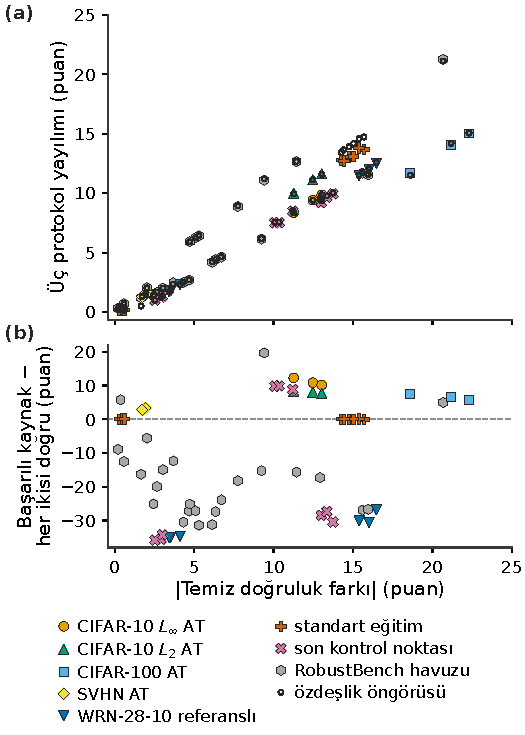
\includegraphics[width=\columnwidth]{../figures/final_tr/fig_spread_clean_gap.pdf}
\caption{Ölçülen $60$ model çiftinin tamamında protokol yayılımının mutlak temiz doğruluk farkına göre değişimi. (a) Asimetrinin koşulsuz, hedef doğru ve her ikisi doğru protokolleri üzerindeki yayılımı; küçük içi boş halkalar aynı çift için $p=1$ alınarak hesaplanan Denklem~\eqref{eq:raw_identity} öngörüsünü gösterir. (b) Aynı çiftlerde başarılı kaynak eksi her ikisi doğru asimetrisi, yani üç protokollü yayılımın dışarıda bıraktığı terim. İşaretçiler her ayarın çekişmeli eğitilmiş çiftlerini, bunların WideResNet-28-10 referansıyla eşleşmelerini, son kontrol noktasındaki aynı çiftleri, standart eğitilmiş çiftleri ve RobustBench havuzunu ayırır; çiftler modelleri paylaştığı için uydurma doğrusu çizilmemiştir.}
\label{fig:spread_clean_gap}
\end{figure}

% REF: Yayilim - temiz fark iliskisi (tum ciftler): uc protokol egim +0.796, r 0.9571, grup-birak +0.767; +0.855;
%      57/60 esitlik; ozdeslik paritesi en buyuk 1.09, ortalama 0.13; dort protokol +0.092, r 0.0532
Şekil~\ref{fig:spread_clean_gap} ilişkiyi ölçülen her çifte genişletmektedir. Bu çiftler üç veri kümesinin ve iki tehdit modelinin çekişmeli eğitilmiş çiftleri, bunların WideResNet ile eşleşmeleri, son kontrol noktasındaki aynı CIFAR-10 çiftleri (Bölüm~\ref{subsec:selection}), standart eğitilmiş çiftler ve Bölüm~\ref{subsec:external}'teki dış havuzdur; toplam $60$ sırasız çift söz konusudur. CIFAR-100 ve $L_2$ ayarlarının WideResNet eşleşmeleri dahil edilmemiş, havuzun ilk CIFAR-10 eğitim çiftiyle çakışan üç çifti ise çekişmeli eğitilmiş gruplarda bir kez sayılmıştır. Üç protokollü yayılım farkla birlikte artmakta (eğim $+0{,}796$, Pearson $r = 0{,}957$; herhangi bir grup dışarıda bırakıldığında $+0{,}767$ ile $+0{,}855$ arasında) ve $60$ noktanın $57$'sinde koşulsuz eksi hedef doğru farkına eşit olmaktadır. İçi boş halkalarla çizilen Denklem~\eqref{eq:raw_identity} öngörüsü her noktayı $1{,}09$ puan içinde izlemekte (ortalama mutlak sapma $0{,}13$), en büyük sapmalar ise $p$'nin birden en uzak olduğu standart eğitilmiş hedeflerde görülmektedir (Bölüm~\ref{subsec:external}). Dört protokollü yayılım farkı izlememekte (eğim $+0{,}092$, $r = 0{,}053$) ve temiz doğrulukları neredeyse eşit gürbüz çiftlerde büyük kalmaktadır. Bu yayılım Carmon vd.~\cite{carmon2019unlabeled} ile Gowal vd.'nin~\cite{gowal2020uncovering} iki WideResNet-28-10 kontrol noktasında ($0{,}21$ puan fark) $9{,}03$, XCiT-S12 ile Gowal vd.\ modelinde ($0{,}58$) $12{,}73$, bu çalışmanın ResNet-18 modeli ile Engstrom vd.'nin~\cite{engstrom2019robustness} ResNet-50 modelinde ($1{,}66$) ise $17{,}50$ puandır. Bunun nedenini (b) paneli göstermektedir. Başarılı kaynak terimi farkla ilişkisizdir; PGD-10 gürbüz doğrulukları sıfıra yakın olduğu için hemen her kaynak saldırısının başarılı olduğu standart eğitilmiş çiftlerde sıfıra yakın, gürbüz modeller arasında ise büyüktür ve iki işaretten birini taşımaktadır. Çiftler modelleri ve koşumları paylaştığı için bu eğimler havuzu betimlemekte, hiçbir şeyi sınamamaktadır.

% REF: Yayilim - temiz fark iliskisi, grup araliklari (SVHN uc protokol 1.30; 1.49)
% REF: Standart egitimli hedeflerde oncul p, cift turune gore ozet (0.47+-0.16; 0.19+-0.02)
Eşlenmiş çift öngörüsü ayrı bir bulgu değil, özdeşliğin bir sonucudur. Koşulsuz, hedef doğru ve her ikisi doğru kestirimleri temiz hatalarla ölçeklenen terimler üzerinden ayrıştığından, temiz doğrulukta eşlenmiş bir çiftin mimarisi ne olursa olsun bu kestirimleri birbirine yakın bırakması beklenir. Verilerin katkısı, öngörünün gerektirdiği üç ölçülmüş olgudur. İncelenen her çekişmeli eğitilmiş hedefte $p$ en az $0{,}984$'tür, her ikisi doğru kestirimi $60$ noktanın $57$'sinde diğer ikisinin arasında yer almaktadır ve başarılı kaynak terimi farka bağlı değildir. Buna uygun olarak $1{,}84$ puanlık farkla SVHN'in iki çiftinde üç protokollü yayılım $1{,}49$ ve $1{,}30$ puandır; aralarında $0{,}47\pm0{,}16$ puan bulunan standart eğitilmiş ResNet-18 ile WideResNet-28-10 çiftinde ise dört protokolün tamamı $0{,}19\pm0{,}02$ puan içindedir (Bölüm~\ref{subsec:external}). CIFAR-10'daki $15$ puanlık aralığın temiz doğruluk farkından gelen kısımları, yani özdeşlik terimi ve onaylanan ikili içindeki uzaklık, temiz doğrulukta eşlenmiş çiftlerde küçülmelidir; yukarıdaki gürbüz çiftlerin gösterdiği gibi başarılı kaynak fazlasının küçülmesi ise gerekmemektedir.

% ----------------------------------------------------------------------------
% E. Standart egitilmis hedefler ve dis havuz
% ----------------------------------------------------------------------------
\subsection{Standart Eğitilmiş Hedefler ve Dış Model Havuzu}
\label{subsec:external}

% REF: Standart egitimli hedeflerde oncul p (temiz ciftler); RobustBench havuzu (8 model, tohum 42)
\begin{sloppypar}
Bu çalışmanın çekişmeli eğitilmiş çiftinin yanıtlayamadığı iki soru kalmaktadır. Bunlar öncül $p$'nin transfer çalışmalarının çoğunun saldırdığı rejim olan standart eğitilmiş hedeflerde sağlanıp sağlanmadığı ve eşlenmiş çift öngörüsünün başkalarının eğittiği modellerde tutup tutmadığıdır. İki soru da yeni bir eğitim yapılmadan yanıtlanmıştır. İlk olarak üç eğitim çiftinin, çekişmeli ince ayarın başlangıç noktaları olan temiz eğitilmiş ResNet-18 ve ViT-Tiny kontrol noktaları, RobustBench~\cite{croce2021robustbench} üzerinden dağıtılan standart eğitilmiş WideResNet-28-10 (tanımlayıcı \texttt{Standard}) ile birleştirilerek çift başına bir $3\times3$ matris kurulmuştur. İkinci olarak sekiz modelli bir CIFAR-10 havuzu, ilk çiftin çekişmeli eğitilmiş ResNet-18 ve ViT-Tiny modellerini, standart eğitilmiş WideResNet'i ve RobustBench tanımlayıcılarıyla anılan beş gürbüz RobustBench kontrol noktasını bir araya getirmektedir: bir PreAct ResNet-18 (\texttt{Wong2020Fast})~\cite{wong2020fast}, bir ResNet-50 (\texttt{Engstrom2019Robustness})~\cite{engstrom2019robustness}, etiketsiz veriyle eğitilmiş bir WideResNet-28-10 (\texttt{Carmon2019Unlabeled})~\cite{carmon2019unlabeled}, dikkati evrişim bileşenleriyle birleştiren bir XCiT-S12 (\texttt{Debenedetti2022Light\_XCiT-S12})~\cite{debenedetti2023light} ve önceki bölümlerin WideResNet-28-10 referansı~\cite{gowal2020uncovering}. Her yöne tam test kümesinde, örnek bazında kayıtla $\eps=8/255$ bütçeli PGD-10 saldırısı uygulanmış; dört protokol, $p$ ve $p=1$ artığı bu kayıtlardan hesaplanmıştır (Tablo~\ref{tab:external_pool}).
\end{sloppypar}

% REF: Standart egitimli hedeflerde oncul p, hedef turune gore (tum yonler 0.8774-1.0000; Standard WRN hedef 0.8774-0.9962;
%      ViT temiz hedef 0.9231-0.9338; artik en buyuk 1.58)
% REF: RobustBench havuzu (56 yon, p 0.9330-1.0000; artik en buyuk 0.35; AT hedeflerde p en kucuk 0.9846)
% REF: Secim kuralinin asimetriye etkisi, B (son kontrol noktasi p en kucuk 0.9915; artik en buyuk 0.20)
Standart eğitilmiş hedeflerde öncül zayıflamaktadır. Üç temiz matrisin $18$ köşegen dışı yönünde $p$ değeri $0{,}877$ ile $1{,}000$ arasında değişmektedir; en düşük değerler standart eğitilmiş WideResNet hedef olduğunda görülmekte ($0{,}877$ ile $0{,}996$), temiz ViT-Tiny hedefinde ise $p$ $0{,}923$ ile $0{,}934$ arasında kalmaktadır. Bu durumda $p=1$ biçimi koşulsuz oranı, üç hedef içinde temiz hatası en büyük olan ViT-Tiny hedefinde $1{,}58$ puana kadar ıskalamaktadır. Orada Denklem~\eqref{eq:raw_identity} bir üst sınırdır ve kullanılması gereken düzeltme, ölçülmüş $p$ ile genel biçim olan Denklem~\eqref{eq:general_identity}'dir. Sekiz hedeften yedisinin çekişmeli eğitilmiş olduğu havuzda her çekişmeli eğitilmiş hedefte $p\geq0{,}984$, standart eğitilmiş hedefte $p\geq0{,}933$'tür ve $p=1$ artığı $56$ yönün tamamında $0{,}35$ puan içinde kalmaktadır; bu çalışmanın çiftlerinin son kontrol noktasında ise artık $0{,}20$ puanı aşmamaktadır (Bölüm~\ref{subsec:selection}).

% REF: Standart egitimli hedeflerde oncul p, cift basina dort protokol asimetrisi ve cift turune gore ozet
Standart eğitilmiş matrisler eşlenmiş çift öngörüsünü farklı bir eğitim rejiminde de sınamaktadır. Temiz ResNet-18 ile standart WideResNet temiz doğrulukta $0{,}47\pm0{,}16$ puan ayrışmakta ve dört protokol kestirimleri $0{,}19\pm0{,}02$ puan içinde uyuşmaktadır (ilk çiftte $-3{,}35$, $-3{,}54$, $-3{,}51$ ve $-3{,}50$). Yaklaşık $15$ puan ayrışan iki eşlenmemiş çiftte ($15{,}16\pm0{,}48$ ve $14{,}69\pm0{,}60$) yayılım $13{,}25\pm0{,}34$ ve $13{,}08\pm0{,}60$ puandır ve her koşuda koşulsuz protokol diğer üçünün bildirdiği işareti tersine çevirmektedir; temiz ResNet-18 ve ViT-Tiny için koşulsuz protokol $+7{,}81$ ile $+10{,}09$ puan verirken hedef doğru protokolü $-5{,}22$ ile $-3{,}56$ puan vermektedir. Dolayısıyla standart eğitim altında bu çalışmanın ResNet-18 ve ViT-Tiny modelleri her koşullu protokolde ters yönü, yani Mahmood vd.'nin bildirdiği yönü göstermektedir (her ikisi doğru $-3{,}02$ ile $-1{,}30$), ancak onların mekanizmasını göstermemektedir. Toplamsal uydurma (Tablo~\ref{tab:source_target}) temiz ViT-Tiny modelini açık ara en zayıf kaynak olarak tutmakta (kaynak farkı $+69{,}18\pm2{,}31$) ve işareti hedef terimi üzerinden çevirmektedir ($-75{,}05\pm1{,}72$); temiz ViT-Tiny, zayıf bir kaynak olduğundan da daha zor bir hedeftir. Standart WideResNet iki karşıtlığı da doğrudan göstermektedir; ResNet'te üretilen örneklerin $\%81{,}40$'ı, ViT'te üretilenlerin ise $\%13{,}60$'ı tarafından kandırılmakta, kendisi de ResNet'i $\%84{,}05$, ViT'i $\%7{,}62$ oranında kandırmaktadır.

% REF: RobustBench havuzu (28 cift; temiz fark 0.21-20.68; uc protokol +0.872 [+0.534; +1.274], r 0.9438;
%      dort protokol +0.559 [-0.205; +4.582]; isaret donen 1/28; ViT_Tiny_AT/Standard -6.72 / +14.53, fark 20.68;
%      Carmon2019/Gowal2020: fark 0.21, uc 0.32, dort 9.03; toplamsal: R2 0.8955, kaynak etkileri, hedef etkileri)
Temiz farkları $0{,}21$ ile $20{,}68$ puan arasında değişen $28$ çiftli havuzda üç protokollü yayılım temiz farkın puanı başına $0{,}872$ puan artmakta (model dışarıda bırakmalı bootstrap aralığı $[+0{,}534;\ +1{,}274]$, $r = 0{,}944$), dört protokollü yayılım ise güvenilir bir ilişki göstermemektedir ($+0{,}559$, $[-0{,}205;\ +4{,}582]$). İşaret protokoller arasında $28$ çiftin yalnızca birinde, bu çalışmanın çekişmeli eğitilmiş ViT-Tiny modeli ile standart eğitilmiş WideResNet çiftinde değişmektedir; bu çift aynı zamanda en geniş farka sahip çifttir ($20{,}68$ puan; koşulsuz $-6{,}72$, hedef doğru $+14{,}53$). Temiz doğrulukları neredeyse eşit gürbüz modeller eşlenmiş çift öngörüsünü ve onun sınırını aynı anda doğrulamaktadır. Carmon vd.\ ile Gowal vd.'nin aralarında $0{,}21$ puan bulunan iki gürbüz WideResNet-28-10 kontrol noktasında üç protokollü yayılım $0{,}32$, dört protokollü yayılım ise $9{,}03$ puandır. Havuzun hedef doğru matrisine yapılan toplamsal uydurma ($56$ hücrede $R^2 = 0{,}8955$) bu çalışmanın ViT-Tiny modelini çekişmeli eğitilmiş en zayıf kaynak olarak konumlandırmakta (kaynak etkisi $-4{,}87$, diğer gürbüz modellerde $+2{,}94$ ile $+3{,}65$), hedef etkisini ise gürbüz modellerin aralığı ($-4{,}26$ ile $+2{,}76$) içinde $-0{,}63$ olarak vermektedir. Evrişim bileşenli bir dikkat modeli olan gürbüz XCiT-S12, CNN'ler kadar güçlü bir kaynaktır ($+3{,}06$). Bölüm~\ref{subsec:source_target}'deki kaynak etkisi bu nedenle bir aile olarak dönüştürücülerin değil, sıfırdan düşük bir temiz doğruluğa eğitilmiş bu ViT-Tiny modelinin özelliği olarak okunmalıdır; havuzdaki tek gürbüz dikkat tabanlı model daha fazlasını söylemeye yetmemektedir.

% REF: tablo hucreleri: "Standart egitimli hedeflerde oncul p", "RobustBench havuzu",
%      "Secim kuralinin asimetriye etkisi" B, ozdeslik_kontrol.json (36 yon, 0.41)
\begin{table}[!t]
\centering
\caption{Denklem~\eqref{eq:general_identity}'deki öncül $p$ ve bu çalışmanın çekişmeli eğitilmiş çifti dışında eşlenmiş çift öngörüsü (CIFAR-10, PGD-10, $\eps$=8/255, tam test kümesi). Üst blok: köşegen dışı yönler üzerinden hedef türüne göre $p$ ve $p=1$ biçiminin puan cinsinden en büyük mutlak hatası (``--'': hedef türü başına saklanmamıştır). Orta blok: her biri bir eğitim çiftinin temiz ResNet-18 ya da ViT-Tiny modeli veya RobustBench'in standart eğitilmiş WideResNet-28-10 modeli olan standart eğitilmiş çiftler, üç çift üzerinden ortalama$\pm$std; işaret dönmesi dört protokolün işarette uyuşmadığını gösterir. Alt blok: sekiz modelli havuzun $28$ çifti üzerinde protokol yayılımının mutlak temiz doğruluk farkına göre eğimi; çiftler modelleri paylaştığı için aralık model dışarıda bırakmalı bootstrap ile verilmiştir.}
\label{tab:external_pool}
\footnotesize
\setlength{\tabcolsep}{3pt}
\begin{tabular}{lccc}
\toprule
\textbf{Hedef} & \textbf{Yön} & \textbf{$p$ aralığı} & \textbf{Maks.\ $|$artık$|$} \\
\midrule
AT hedefleri, $3\times3$ & 36 & 0,9890--1,0000 & 0,41 \\
AT hedefleri, son k.\,n. & 18 & 0,9915--1,0000 & 0,20 \\
Temiz ViT-Tiny & 6 & 0,9231--0,9338 & 1,58 \\
Temiz ResNet-18 & 6 & 0,8961--1,0000 & 0,51 \\
Standart WRN-28-10 & 6 & 0,8774--0,9962 & 0,64 \\
Havuz, AT hedefleri & 49 & 0,9846--1,0000 & -- \\
Havuz, standart WRN & 7 & 0,9330--0,9962 & -- \\
Havuz, tüm hedefler & 56 & 0,9330--1,0000 & 0,35 \\
\midrule
\textbf{Std.\ eğitilmiş çift} & \textbf{$|$Temiz fark$|$} & \textbf{Yayılım} & \textbf{İşaret dön.} \\
\midrule
ResNet-18 / WRN & 0,47$\pm$0,16 & 0,19$\pm$0,02 & 0/3 \\
ResNet-18 / ViT-Tiny & 15,16$\pm$0,48 & 13,25$\pm$0,34 & 3/3 \\
ViT-Tiny / WRN & 14,69$\pm$0,60 & 13,08$\pm$0,60 & 3/3 \\
\midrule
\textbf{Havuz yayılımı} & \textbf{Eğim} & \textbf{\%95 aralık} & \textbf{$r$} \\
\midrule
Üç protokol & $+$0,872 & [$+$0,534; $+$1,274] & 0,944 \\
Dört protokol & $+$0,559 & [$-$0,205; $+$4,582] & 0,350 \\
İşaret dön.\ (4 prot.) & \multicolumn{3}{c}{1/28 çift} \\
\bottomrule
\end{tabular}
\end{table}

% ----------------------------------------------------------------------------
% F. Kontrol noktasi secimi
% ----------------------------------------------------------------------------
\subsection{Kontrol Noktası Seçimi ve Asimetri}
\label{subsec:selection}

Sabit bir yörüngeden son kontrol noktasını seçen çevrimdışı kural, gürbüz aşırı öğrenme bu seçimi çekişmeli eğitimde sonuç doğurucu kılsa da~\cite{rice2020overfitting} genellikle örtük bırakılmaktadır. Bir eğitim yörüngesi sabit tutulup yalnızca son kontrol noktasının nasıl seçildiği, yani doğrulama bölmesi, erken durdurma sabrı ve argmaks öncesinde doğrulama eğrisinin yumuşatılıp yumuşatılmadığı değiştirildiğinde (on sekiz bileşim) raporlanan PGD-10 doğruluğu ResNet'te tohum başına $2{,}62$ ile $2{,}85$, ViT'te $1{,}58$ ile $2{,}09$ puan oynamaktadır. Bu hücrelerde diskteki ağırlıklar özdeştir ve yalnızca içlerinden birini seçen kural farklıdır. Bu yayılımın yaklaşık yarısı üç boyuttan yalnızca birinden gelmektedir. Argmaks öncesinde doğrulama eğrisini yumuşatmak, üç ResNet koşumunun üçünde ve üç ViT koşumunun ikisinde test PGD-10 doğruluğunu monoton biçimde düşürmektedir; yani sistematik olarak daha kötü bir kuraldır. Çalışmaların fiilen değiştirdiği bölme ve sabır seçimleriyle sınırlandığında yayılım ResNet'te tohum düzeyi standart sapmanın $1{,}09$ katına, ViT'te $1{,}42$ katına inmektedir. Bu yayılım mutlak birimlerle raporlanmakta ve bilinçli olarak tohum düzeyi yayılıma oran biçiminde verilmemektedir; çünkü o oran on sekiz hücreden hangisinin referans alındığına bağlıdır ve on sekizinin tamamı tarandığında ResNet'te $0{,}67$ ile $3{,}38$, ViT'te $0{,}63$ ile $7{,}38$ arasında değişerek bazı referanslarda karşılaştırmayı tersine çevirmektedir.

CIFAR-100 koşuları bir karşı ağırlık sağlamaktadır. Bu çalışmanın protokolünün seçtiği epok üç ResNet tohumu arasında $25$ epok kaymakta, buna karşılık ortaya çıkan test PGD-10 standart sapması $0{,}32$ puanda kalmaktadır. Seçim \emph{yolu} oynak, seçilen \emph{sonuç} ise kararlı olmuştur; bunlardan hangisinin gerçekleşeceği mimariye değil yörüngenin platosuna bağlıdır.

% REF: Secim kuralinin asimetriye etkisi, B. Son kontrol noktasi ve fark ozeti
%      (temiz fark 12.26+-0.90 -> 10.55+-0.59, degisim -1.71+-0.84; dort yayilim 15.01+-0.84 -> 12.84+-0.34,
%       degisim -2.16+-0.93; uc yayilim 9.21+-0.76 -> 7.84+-0.56; tc +4.36+-0.44 -> +4.64+-0.56;
%       ss +19.37 -> +17.48; p en kucuk 0.9915; artik en buyuk 0.20)
Seçim kuralı, yayılımın bağlı olduğu temiz doğruluk farkını belirlediği için transfer asimetrisine de ulaşmaktadır. Üç eğitim çiftinin seçilen kontrol noktası yerine son kontrol noktasında, yani erken durdurmanın eğitimi sonlandırdığı epokta yeniden puanlanması (ResNet'ler için $71$, $76$ ve $77$, ViT'ler için $45$, $38$ ve $39$; seçilen $51$, $56$, $57$ ve $25$, $18$, $19$. epoklardan yirmi epok sonra) temiz farkı $12{,}26\pm0{,}90$ puandan $10{,}55\pm0{,}59$ puana (değişim $-1{,}71\pm0{,}84$), dört protokollü yayılımı ise $15{,}01\pm0{,}84$ puandan $12{,}84\pm0{,}34$ puana (değişim $-2{,}16\pm0{,}93$) daraltmaktadır; üç protokollü yayılım da $9{,}21\pm0{,}76$'dan $7{,}84\pm0{,}56$'ya inmektedir. Hedef doğru asimetrisi neredeyse yerinden oynamamakta ($+4{,}36\pm0{,}44$'e karşı $+4{,}64\pm0{,}56$), başarılı kaynak kestirimi $+19{,}37$'den $+17{,}48$'e düşmekte, dört protokolün tamamı her çiftte CNN$\rightarrow$ViT işaretini korumakta ve öncül önceki gibi sağlanmaktadır ($p\geq0{,}9915$, $p=1$ artığı en çok $0{,}20$ puan).

% REF: Secim kuralinin asimetriye etkisi, A. Saklanan egitim yorungeleri (CIFAR-10 temiz fark secilen 10.59-12.65,
%      son 11.83-13.83; yayilim Delta ResNet -1.53+-1.15, ViT -0.03+-1.15; tc Delta ViT +2.53+-0.15;
%      CIFAR-100 yayilim Delta ResNet -1.84+-0.94, ViT +0.84+-0.24)
Saklanan eğitim yörüngeleri eğitim boyunca aynı tabloyu vermektedir. Bu yörüngeler ana çiftlerin seçilen kontrol noktalarından değil, aynı tohumlarla yapılan CIFAR-10 yeniden eğitim koşularından ve doğrudan CIFAR-100 koşularından gelmekte ve yaklaşık her on epokta bir kaydedilmektedir. CIFAR-10'da bu yeniden eğitim koşuları temiz farkı hem seçilen hem son epokta $10{,}59$ puanda ya da üstünde tutmaktadır; dolayısıyla seçim farkı yaklaşık $1{,}7$ puan oynatmakta, ancak ortadan kaldırmamaktadır. Farkın tam büyüklüğü ise seçime duyarlıdır. Bir çiftin bir üyesini seçilen epoğundan son epoğuna taşımak dört protokollü yayılımı ResNet taşındığında $-1{,}53\pm1{,}15$ puan, ViT taşındığında $-0{,}03\pm1{,}15$ puan değiştirmekte, ViT'in taşınması ise hedef doğru asimetrisini $+2{,}53\pm0{,}15$ puan kaydırmaktadır; CIFAR-100'de yayılım $-1{,}84\pm0{,}94$ ve $+0{,}84\pm0{,}24$ puan değişmektedir. Seçim kuralı böylece asimetrinin düzeyini yaklaşık iki buçuk puana, yayılımını ise yaklaşık iki puana kadar oynatmakta, ancak yönü ya da büyüklük mertebesini değiştirmemektedir. Bu kuralın yöntem bölümünde belirtilmesi gerekir.

% ----------------------------------------------------------------------------
% G. Uc okuma (gradyan, dikkat, TGR tek alt bolumde)
% ----------------------------------------------------------------------------
\subsection{Doğrudan Ölçümde Ayakta Kalmayan Üç Okuma}
\label{subsec:readings}

Mimari karşılaştırmaları transfer asimetrisinin ötesinde üç okumayı da akla getirmektedir: CNN gradyanlarının mekansal olarak daha lokalize olduğu, çekişmeli pertürbasyonun ViT dikkatini bozduğu ve ViT'e özgü transfer saldırılarının ViT kaynaklı transferi iyileştirdiği. Her biri doğrudan ölçülmüş, hiçbiri bu rejimde geçerli çıkmamış ve aynı ölçümler iki davranışsal farkı ayakta bırakmıştır.

% ----------------------------------------------------------------------------
% G.1 Gradyan seyrekligi ve mekansal lokalite
% ----------------------------------------------------------------------------
\subsubsection{Mekansal lokalite olmadan gradyan seyrekliği}
\label{subsec:gradient}
\label{subsubsec:spatial}

\begin{table}[!t]
\centering
\caption{Örnek başına kayıp gradyanlarından hesaplanan gradyan karakteristikleri (koşu başına $n$=500 test örneği; üç koşu üzerinden ortalama$\pm$std). Kalın yazı, çekişmeli eğitilmiş iki modelden büyük olanı gösterir; yerel kontrol tek bir kontrol noktası olduğundan standart sapma verilmemiştir.}
\label{tab:gradient}
\footnotesize
\setlength{\tabcolsep}{2.5pt}
\begin{tabular}{lccc}
\toprule
\textbf{Metrik} & \textbf{ResNet-18 AT} & \textbf{ViT-Tiny AT} & \textbf{ViT (yerel)$^\ddagger$} \\
\midrule
Hoyer seyrekliği & \textbf{0,4928}$\pm$0,0120 & 0,4561$\pm$0,0055 & 0,4046 \\
Gini katsayısı & \textbf{0,6498}$\pm$0,0089 & 0,6099$\pm$0,0051 & 0,5712 \\
Maks.\ \%1 altı kesir & \textbf{0,3477}$\pm$0,0210 & 0,2682$\pm$0,0090 & 0,1785 \\
Hizalanma (mutlak) & 0,0378$\pm$0,0009 & \textbf{0,0562}$\pm$0,0004 & 0,0794 \\
Hizalanma (işaretli) & 0,0010$\pm$0,0003 & 0,0004$\pm$0,0001 & -- \\
\bottomrule
\multicolumn{4}{l}{\scriptsize $^\ddagger$CIFAR'a özgü ViT kontrolü ($4\times4$ yama, 5,4M parametre); sabit bölme}\\
\multicolumn{4}{l}{\scriptsize \phantom{$^\ddagger$}protokolünden önceye ait, test kümesinde seçilmiş tek kontrol noktası;}\\
\multicolumn{4}{l}{\scriptsize \phantom{$^\ddagger$}yalnızca büyütme etkisinin işareti için eklenmiştir.}
\end{tabular}
\end{table}

% REF: Gradyan yapisi (Hoyer temiz 0.3467 / 0.3804; hizalanma temiz 0.0293 / 0.0581; Cohen d 0.32-1.23; isaretli en buyuk 0.0014)
CNN girdi gradyanları üç ölçekten bağımsız ölçünün üçünde de ViT gradyanlarından daha seyrektir (Tablo~\ref{tab:gradient}; normlar değerlendirme parti boyuna bağlı olmasın diye örnek başına kayıp gradyanları, hizalanma için tüm $500\times499/2$ örnek çifti üzerinden ortalama mutlak kosinüs) ve sıralama, tohum düzeyi standart sapmalar farktan en az üç kat küçük kalarak her koşuda yeniden üretilmektedir. İki çıkarım biriminin uyuşmadığı tek yer burasıdır ve bu nedenle ikisi de raporlanmaktadır. Aynı 500 örneğin iki modelde de ölçüldüğü koşum içinde örnek başına eşleştirilmiş Wilcoxon testleri üç ölçüde de sıfır hipotezini reddetmektedir (Holm düzeltmeli $p<10^{-11}$, eşleştirilmiş Cohen $d$ 0,32 ile 1,23 arasında). Mimari bir iddianın gerektirdiği birim olan koşum düzeyinde ise üç eşleştirilmiş koşum Gini, \%1 altı kesir ve Hoyer için $0{,}036$, $0{,}042$ ve $0{,}067$ ham $p$ değerleri vermekte, Holm düzeltmesi bunları $0{,}108$'e çıkarmaktadır. Sıralama her koşuda tutarlı ama koşum düzeyinde anlamsız olduğu için anlamlı olarak değil, yeniden üretilebilir olarak raporlanmaktadır. Sıralama çekişmeli eğitimin ürünüdür. Aynı koşuların temiz eğitilmiş karşılıklarında daha seyrek model \emph{ViT'tir} (Hoyer $0{,}380\pm0{,}009$'a karşı $0{,}347\pm0{,}002$); bu durum Chalasani vd.'nin~\cite{chalasani2020concise} çekişmeli eğitilmiş modeller için bildirdiği daha seyrek öznitelik atıflarıyla uyumludur. CIFAR'a özgü ViT kontrolü ise her ölçüde büyütülmüş ViT'ten daha az seyrektir; dolayısıyla sıralama $32\rightarrow224$ büyütmenin artefaktı değildir. Örnekler arası hizalanma mutlak kosinüste ViT'te daha yüksektir; bu fark koşum düzeyinde anlamlılığa ulaşmakta ($p=0{,}0009$) ve temiz eğitilmiş çiftte zaten görülmektedir ($0{,}058$'e karşı $0{,}029$). \emph{İşaretli} ortalama kosinüs ise iki modelde de sıfıra yakındır (her koşumda $\leq0{,}0014$); yani örnekler duyarlılık eksenlerini paylaşmakta, ancak tutarlı bir yönü paylaşmamaktadır.

\begin{table}[!t]
\centering
\caption{Girdi gradyanlarının mekansal lokalitesi (koşu başına $n$=500 örnek; üç koşu üzerinden ortalama$\pm$std). Eşleştirilmiş farklar aynı örnekler üzerinde hesaplanır. Çıkarım koşum düzeyindedir: $p$, üç koşumun ortalama farkları üzerinde tek örneklem $t$ testidir ve dört ölçüye Holm düzeltmesi uygulanmıştır; böylece çıkarımın birimi iddianın birimiyle eşleşir. Düşük alan ve entropi daha lokalize, yüksek Moran's $I$ daha kümeli demektir.}
\label{tab:spatial}
\scriptsize
\setlength{\tabcolsep}{1.6pt}
\begin{tabular}{lcccc}
\toprule
\textbf{Ölçüt} & \textbf{ResNet-18} & \textbf{ViT-Tiny} & \textbf{Fark (R$-$V)} & \textbf{$p$ (Holm)} \\
\midrule
\%50 enerji alanı & 0,0378$\pm$0,0017 & 0,0397$\pm$0,0010 & $-$0,0019$\pm$0,0027 & 0,54 \\
\%90 enerji alanı & 0,2345$\pm$0,0078 & 0,2570$\pm$0,0067 & $-$0,0224$\pm$0,0133 & 0,40 \\
Mekansal entropi (nat) & 5,2014$\pm$0,0387 & 5,2524$\pm$0,0197 & $-$0,0509$\pm$0,0580 & 0,54 \\
Moran's $I$ & 0,4141$\pm$0,0132 & 0,3941$\pm$0,0024 & $+$0,0200$\pm$0,0156 & 0,47 \\
\bottomrule
\end{tabular}
\end{table}

% REF: Tablo 9 ek sutunlari (Holm p 0.402-0.535; kosum degerleri: alan50 ve entropi isaret degistiriyor)
Seyreklik kaç gradyan bileşeninin büyük olduğunu saymakta, ancak bu bileşenlerin görüntüde bir arada durup durmadığını, yani gradyanları lokalize olarak betimleyen ifadenin ileri sürdüğü şeyi söylememektedir. Aynı gradyanların kanal toplamı enerji haritası üzerinde dört ölçekten bağımsız betimleyicinin hiçbiri koşum düzeyinde farklılaşmamaktadır (Tablo~\ref{tab:spatial}; Holm düzeltmeli $p$ değerleri $0{,}40$ ile $0{,}54$ arasında). Enerjinin \%90'ını taşıyan alan CNN için görüntü alanının iki yüzde puanı kadar \emph{daha küçük} bir alana işaret etmekte ve dört mekansal sıralamanın ikisi koşumlar arasında işaret değiştirmektedir; seyreklik sıralaması ise her koşuda her ölçüde korunmaktadır. Çekişmeli eğitilmiş CNN gradyanları kütlelerinin daha büyük kısmını daha az piksele yerleştirmekte, ancak bu pikseller ViT'inkilerden mekansal olarak daha kümeli olmamaktadır; bu nedenle bu çalışmanın iddiaları seyreklikle sınırlı tutulmuştur. Şekil~\ref{fig:gradient_analysis} ölçekten bağımsız ölçülerin yakalamadığı örnek başına gradyan normlarının dağılımını eklemektedir; Şekil~\ref{fig:gradient_heatmap}'teki büyüklük haritaları da lokalite olarak değil seyreklik olarak okunmalıdır.

\begin{figure}[!t]
\centering
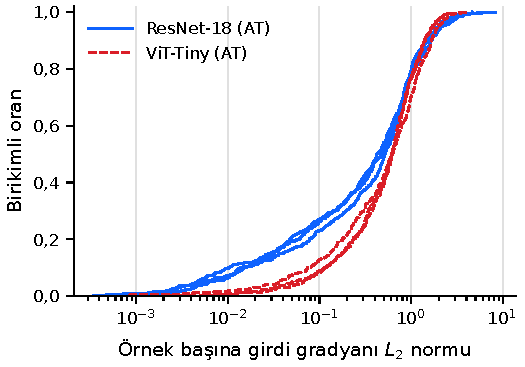
\includegraphics[width=\columnwidth]{../figures/final_tr/fig4b_gradient_distribution.pdf}
\caption{Örnek başına girdi gradyanı $L_2$ normlarının deneysel dağılımı (örnek başına çapraz entropi kaybı, ilk $500$ test görüntüsü, eğitim koşusu başına bir eğri, mimari başına üç koşu; logaritmik eksen). Bu girdilerden dördünün büyüklük haritaları Şekil~\ref{fig:gradient_heatmap}'te verilmektedir.}
\label{fig:gradient_analysis}
\end{figure}

\begin{figure}[!t]
\centering
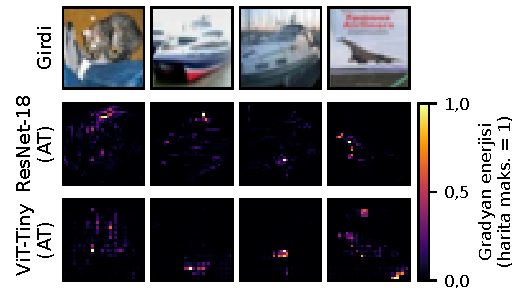
\includegraphics[width=\columnwidth]{../figures/final_tr/fig4_gradient_comparison.pdf}
\caption{Aynı test görüntüleri için iki modelde girdi gradyanı büyüklük haritaları (tohum çifti 1; ilk dört test görüntüsü; her harita kendi en büyük değerine ölçeklendiğinden büyüklükler paneller arasında karşılaştırılamaz). CNN gradyanları kütlelerinin daha büyük kısmını daha az bileşene yerleştirmektedir (Tablo~\ref{tab:gradient}). Tablo~\ref{tab:spatial} bu durumun mekansal dizilişte bir farkla birlikte gelmediğini göstermektedir; bu yüzden paneller lokalite olarak değil seyreklik olarak okunmalıdır.}
\label{fig:gradient_heatmap}
\end{figure}

% ----------------------------------------------------------------------------
% G.2 Dikkat ve oznitelik kaymasi
% ----------------------------------------------------------------------------
\subsubsection{Dikkat entropisi ve öznitelik kayması}
\label{subsec:attention}

\begin{table}[!t]
\centering
\caption{Her modelin kendi beyaz kutu PGD-10 saldırısı altında blok bazlı temizden çekişmeliye kosinüs benzerliği (koşu başına $n$=1000; üç koşu ortalaması). Tüm özetler artık blok çıkışında alınmıştır, böylece ViT ve CNN sütunları eşdeğer noktalarda ölçülmektedir; ViT sütunları yalnızca bir bloğun jetonlarının nasıl toplandığında ayrışır. MLP alt-blok çıkışına ait değerler metinde verilmiştir. Koşumlar arası standart sapma ViT sütunlarında en çok 0,0061, ResNet sütununda en çok 0,0181'dir (aşama 4, blok 1); kalın yazı her sütunun en küçük değerini gösterir.}
\label{tab:feature_degradation}
\footnotesize
\setlength{\tabcolsep}{2.5pt}
\begin{tabular}{lccc@{\hspace{9pt}}lc}
\toprule
\multicolumn{4}{c}{\textbf{ViT-Tiny AT}} & \multicolumn{2}{c}{\textbf{ResNet-18 AT}} \\
\cmidrule(lr){1-4} \cmidrule(lr){5-6}
\textbf{Blok} & \textbf{CLS} & \textbf{Yama ort.} & \textbf{Tüm jetonlar} & \textbf{Aşama.blok} & \textbf{Kosinüs} \\
\midrule
1 & 0,9993 & 0,9980 & 0,9927 & 1.1 & 0,9951 \\
2 & 0,9950 & 0,9959 & 0,9901 & 1.2 & 0,9918 \\
3 & 0,9902 & 0,9940 & 0,9881 & 2.1 & 0,9879 \\
4 & 0,9873 & 0,9919 & 0,9861 & 2.2 & 0,9853 \\
5 & 0,9845 & 0,9904 & 0,9847 & 3.1 & 0,9753 \\
6 & 0,9814 & 0,9894 & 0,9835 & 3.2 & 0,9607 \\
7 & 0,9782 & 0,9885 & 0,9826 & 4.1 & \textbf{0,8777} \\
8 & 0,9743 & 0,9875 & 0,9816 & 4.2 & 0,9108 \\
9 & 0,9703 & \textbf{0,9870} & 0,9809 & & \\
10 & 0,9661 & 0,9872 & 0,9805 & & \\
11 & \textbf{0,9604} & 0,9874 & \textbf{0,9803} & & \\
12 & 0,9663 & 0,9915 & 0,9837 & & \\
\bottomrule
\end{tabular}
\end{table}

% REF: C4: oznitelik kaymasi ve attention (CLS 0.9604 blok 11; yama 0.9870 blok 9; oran 3.05;
%      MLP alt-blok: CLS 0.9343 blok 10, yama 0.9840 blok 8); ResNet layer4.0 0.8777+-0.0181, -13.14+-1.89%; layer4.1 0.9108+-0.0060
Çekişmeli hasarın derinlik boyunca nerede biriktiği iki mimaride farklıdır (Tablo~\ref{tab:feature_degradation}; artık blok çıkışları, koşu başına $n=1000$) ve bu ölçüm temiz eğitilmiş ViT'lerin katman bazlı analizlerini~\cite{raghu2021vision} çekişmeli eğitilmiş ortama taşımaktadır. ViT'te kayma kademelidir ve yalnızca yönü değiştirmektedir. Benzerlik 11. bloktaki minimuma kadar azalmakta ve çıkışta hafifçe toparlanmakta, öznitelik normları ise temiz değerlerinin \%0,45'i içinde kalmaktadır. CNN'de ise hasar yoğunlaşmıştır; son aşamanın ilk bloğu $-\%13{,}14\pm1{,}89$'luk bir norm daralmasıyla $0{,}8777\pm0{,}0181$'e düşmekte, son blok ise temsili kısmen onarmaktadır ($0{,}9108\pm0{,}0060$). Ölçülen ViT profili jeton agregasyonuna bağlıdır. Minimumlarında CLS yolu yama jetonu ortalamasının yaklaşık üç katı kaymakta ($0{,}9604$'e karşı $0{,}9870$; $1-\cos$ cinsinden oran $3{,}05$) ve minimumlar farklı derinliklerde (blok 11 ve 9) bulunmaktadır; artık blok çıkışı yerine MLP alt-blok çıkışında okunduğunda minimumlar blok 10'da $0{,}9343$'e ve blok 8'de $0{,}9840$'a kaymaktadır. Farklı makalelerden katman bazlı kayma eğrileri ancak hem agregasyon hem de tensör belirtildiğinde karşılaştırılabilir.

% REF: Dikkat entropisi TOST ve devrilen/devrilmeyen kosinus (12/12; en buyuk p 0.00611; en buyuk |degisim| 0.0045;
%      temiz entropi 4.613-5.105; devrilen/devrilmeyen ViT 0.9895/0.9877, p 0.2010; ResNet 0.9058/0.9143, p 0.0804)
% REF: Dikkat entropisi ve CLS dikkat yer degistirmesi (TV 0.0276 -> 0.0841)
Dikkat okuması bu ölçümlerde doğrulanmamaktadır. Çekişmeli pertürbasyon CLS dikkat dağılımının entropisini değiştirmemektedir. Katman başına en büyük ortalama değişim $0{,}0045$ nat iken temiz katman ortalamaları $4{,}61$ ile $5{,}11$ nat arasındadır; ölçünün ölçeğinden sabitlenen $\pm0{,}05$ nat marjıyla üç koşum üzerinden yapılan koşum düzeyi TOST, $12$ katmanın tamamında eşdeğerliği kabul etmekte ve en zayıf sonuç $p=0{,}006$ olmaktadır (Şekil~\ref{fig:feature_degradation}a). Derinlikle büyüyen şey dikkat haritasının yer değiştirmesidir; bu değer ilk katmanda $0{,}028$ toplam varyasyondan son katmanda $0{,}084$'e çıkmaktadır (panel b). Dolayısıyla saldırı dikkati hafifçe yeniden yönlendirmekte, ancak genişletmemekte ya da keskinleştirmemektedir. Şekil~\ref{fig:attention_layers}'teki tek örnekli haritalar yayılmayı değil yeniden yönlendirmeyi göstermektedir ve 8 örneklik daha önceki bir şekil kümesi bu ölçümün desteklemediği bir dikkat etkisi izlenimi vermişti. Öznitelik kayması devrilen ve devrilmeyen örnekleri de ayırmamaktadır; buradaki devrilmeyen grup, modelin temiz girdide zaten yanlış sınıflandırdığı örnekleri de içermektedir. Son blok kosinüsü ViT'te devrilen örneklerde $0{,}9895$, devrilmeyenlerde $0{,}9877$, CNN'de ise $0{,}9058$ ve $0{,}9143$'tür; iki fark da koşum düzeyinde anlamlı değildir (üç koşum üzerinden eşleştirilmiş $t$, $p=0{,}20$ ve $p=0{,}080$), ancak CNN farkı üç koşumun üçünde de aynı işareti taşımaktadır. Yama pertürbasyonları altındaki dikkat kayması etkileri~\cite{gu2022vision} ve dikkat mekanizmasının kendisine yönelik saldırılar~\cite{fu2022patchfool} farklı bir tehdit modeline aittir.

\begin{figure}[!t]
\centering
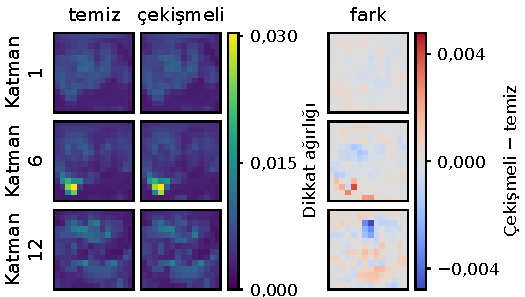
\includegraphics[width=\columnwidth]{../figures/final_tr/fig5_attention_comparison.pdf}
\caption{Çekişmeli saldırı altında ViT katmanları boyunca CLS jetonu dikkat haritaları (softmax sonrası, başlar üzerinden ortalanmış). Her satır farklı bir katmanı (1, 6, 12) gösterir; sütunlar temiz dikkat, çekişmeli dikkat ve farklarıdır ve dikkat sütunları için bir, fark sütunu için bir ortak renk ölçeği kullanılmıştır. Gösterilen tek bir örnektir (ilk test görüntüsü, tohum çifti 1); dikkat yer değiştirmesindeki derinlik eğilimi koşu başına $n$=1.000 örnek üzerinden Şekil~\ref{fig:feature_degradation}(b)'de ölçülmektedir.}
\label{fig:attention_layers}
\end{figure}

\begin{figure}[!t]
\centering
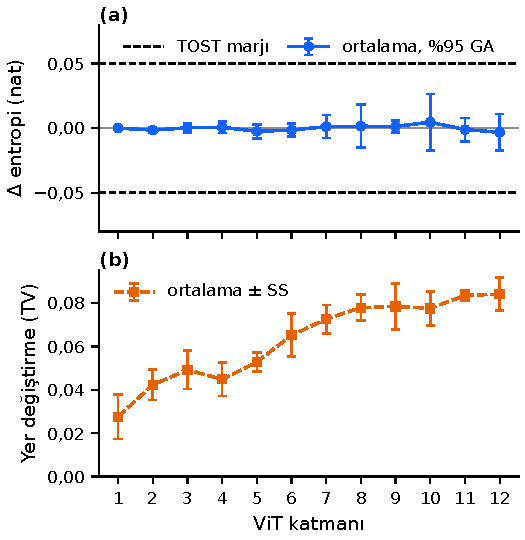
\includegraphics[width=\columnwidth]{../figures/final_tr/fig5b_attention_entropy.pdf}
\caption{(a) Saldırı altında CLS dikkat entropisindeki değişim (çekişmeli eksi temiz), katman başına, üç koşum ortalaması ve \%95 $t$ güven aralıkları; kesikli çizgiler $\pm0{,}05$ nat TOST marjını gösterir ve her aralık bu marjın içindedir. (b) CLS dikkat yer değiştirmesi (temiz ile çekişmeli haritalar arasındaki toplam varyasyon), katman başına, koşumlar üzerinden ortalama$\pm$std. Koşu başına $n$=1.000 örnek; tek örnekli haritalar Şekil~\ref{fig:attention_layers}'te verilmektedir.}
\label{fig:feature_degradation}
\end{figure}

% ----------------------------------------------------------------------------
% G.3 ViT'e ozgu transfer saldirisi
% ----------------------------------------------------------------------------
\subsubsection{ViT'e özgü bir transfer saldırısı}
\label{subsec:tgr}

\begin{table}[!t]
\centering
\caption{Eşleşmiş bütçede Jeton Gradyanı Düzenlileştirme (TGR)~\cite{zhang2023tgr} ve düz momentumlu yinelemeli FGSM (MI-FGSM) altında ViT$\rightarrow$CNN transferi ($L_\infty$, $\eps$=8/255, 10 adım, $\alpha$=2/255; koşu başına $n$=10.000; üç koşu üzerinden ortalama$\pm$std).}
\label{tab:tgr}
\footnotesize
\begin{tabular}{lcc}
\toprule
\textbf{Ölçüt (\%)} & \textbf{TGR} & \textbf{MI-FGSM} \\
\midrule
Kaynakta beyaz kutu (ham) & 51,56$\pm$0,80 & \textbf{66,43}$\pm$0,29 \\
Transfer, hedef doğru & 12,70$\pm$0,41 & \textbf{15,71}$\pm$0,60 \\
Transfer, her ikisi doğru & 7,93$\pm$0,42 & \textbf{10,08}$\pm$0,30 \\
\bottomrule
\end{tabular}
\end{table}

% REF: C2: TGR vs MI-FGSM (66.43 - 51.56 = 14.87; 15.71 - 12.70 = 3.01; 10.08 - 7.93 = 2.15; McNemar p)
Transfer sonuçlarına yöneltilebilecek doğal bir itiraz, dönüştürücü yapısı için tasarlanmış saldırıların daha iyi taşındığı bildirildiğinden ViT'i genel türevlenebilir bir model olarak ele alan gradyan saldırılarının ViT kaynaklı yönü dezavantajlı bıraktığıdır. Geri yayılım sırasında kaynağın dikkat, QKV ve MLP yollarındaki uç değerli jeton gradyanlarını bastıran Jeton Gradyanı Düzenlileştirme (TGR)~\cite{zhang2023tgr} bu itirazı sınamaktadır; bu çalışmadaki uyarlama yöntemi makale boyunca kullanılan bütçeyle CIFAR-10 ViT-Tiny modeline uygulamakta (Bölüm~\ref{subsec:attack_methods}) ve aynı koşuda eşleştirilmiş kontrol olarak düz MI-FGSM üretmektedir. TGR bu rejimde transferi iyileştirmemekte, tersine kötüleştirmektedir (Tablo~\ref{tab:tgr}). Kaynakta 14,9 puanlık beyaz kutu gücünden vazgeçmekte, koşullu transfer ise hedef doğru protokolünde 3,0, her ikisi doğruda 2,2 puan düşmektedir; her ikisi doğru altkümesindeki eşleştirilmiş McNemar testleri her koşuda MI-FGSM lehinedir ($p = 6{,}1\times10^{-10}$, $1{,}1\times10^{-27}$, $7{,}0\times10^{-34}$). Hedefler çekişmeli eğitilmiş, girdiler model içinde büyütülen $32\times32$ CIFAR-10 görüntüleri, kaynak ise 5,7M parametreli bir ViT-Tiny'dir; TGR ise standart eğitilmiş ImageNet ViT'leri için kurulmuştur. Bu nedenle sonuç yöntemi genel olarak değil, bu rejimdeki uyarlamayı sınırlamaktadır. Bu makale açısından sonucun anlamı, CNN$\rightarrow$ViT asimetrisinin mimariden bağımsız saldırıların bir artefaktı olmamasıdır; ViT yönüne dönüştürücüye özgü bir saldırı vermek onu zayıflatmaktadır.

% ----------------------------------------------------------------------------
% H. Varyans kaynaklari
% ----------------------------------------------------------------------------
\subsection{Varyans Kaynakları}
\label{subsec:statistics_results}

Yukarıdaki karşılaştırmaları dört varyans kaynağı ilgilendirmektedir. Saldırı başlatma stokastisitesi ihmal edilebilir düzeydedir; PGD-10'u sabit 1.000 örneklik bir altkümede üç saldırı tohumuyla (42, 123, 456) yeniden koşmak, yükleyici örnekleri karıştırmadığı için temiz doğruluğu hiç değiştirmemekte ve gürbüz doğruluğu CNN'de $0{,}05$, ViT'te $0{,}00$ puanlık standart sapmayla oynatmaktadır. Eğitim koşusu varyansı daha büyük ama yine küçüktür. Mimari başına üç bağımsız koşuda, çekişmeli eğitilmiş çift için standart sapma temiz doğrulukta en çok $0{,}55$, PGD-10'da en çok $0{,}50$ puandır (Tablo~\ref{tab:main_results}).

% REF: Secim kuralinin asimetriye etkisi, B (kosumlar arasi aralik en cok 2.41)
Protokol etkisini doğrudan bu iki sayıyla karşılaştırmak bir ölçek hatası olurdu, çünkü protokol etkisi transfer asimetrisi üzerinde, yukarıdaki iki sayı ise mutlak doğruluk üzerinde ölçülmektedir. Bu nedenle protokol ve eğitim koşusu etkileri \emph{aynı} nicelik olan köşegen dışı asimetri üzerinde ve mutlak birimlerle nicelenmiştir. Sabit bir tohum çiftinde yalnızca koşullama protokolünü değiştirmek asimetriyi $15{,}01\pm0{,}84$ puan oynatmaktadır. Bu değer tohum başına açıklıkların ortalamasıdır; uç protokoller üç tohumda da aynı olduğu için burada protokol ortalamalarının açıklığıyla çakışmakta, uç protokollerin aynı olmadığı CIFAR-100'de ise ondan ayrışmaktadır ($13{,}83$'e karşı $13{,}58$). İki mimariyi yeniden eğitmek aynı asimetriyi en çok $2{,}41$ puanlık bir aralıkta, ölçüldüğü protokole göre $0{,}23$ ile $1{,}27$ puanlık bir standart sapmayla oynatmaktadır (Bölüm~\ref{subsec:transfer}). En çok iki buçuk puana karşı on beş puan, makalenin dayandığı sıralamadır. Kontrol noktası seçim kuralını değiştirmek dört protokollü yayılımı ortalama $2{,}16$ puan oynatmaktadır (Bölüm~\ref{subsec:selection}); bu değer yeniden eğitimin bir protokol içinde asimetriyi oynattığı miktara ($2{,}41$'e kadar) yakındır ve söz konusu sıralamayı bozmamaktadır.

Bu iki yayılımın oranı manşete taşınmamıştır. Üç koşumla payda iki serbestlik derecesi taşıdığından herhangi bir tek oran için $\chi^2$ aralığı çok geniştir; başarılı kaynak protokolünde bu aralık $0{,}8$ ile $9{,}9$ arasında uzanmakta ve biri içermektedir. Duyarlılık olarak raporlandığında oran, yayılım ölçüleri ve referans protokoller boyunca $5{,}2$ ile $32{,}6$ arasında değişmekte, birincil kabul edilen her ikisi doğru protokolündeki benzeri benzeriyle karşılaştırmada ise $28{,}3$ olmaktadır. İki uyarı oranı daha da sınırlamaktadır. En büyük asimetriyi veren protokol aynı zamanda en büyük koşumlar arası standart sapmayı taşımakta, yani pay ile payda bağımsız olmamaktadır; üç koşum tek bir doğrulama bölmesini paylaştığından da payda bölmeler arası varyansı dışarıda bırakmakta ve bu durum oranı bir üst sınır yapmaktadır. Mutlak karşılaştırma iki uyarıdan da etkilenmediği için iddiayı kat değeri değil o taşımaktadır. Dördüncü kaynak olan kontrol noktası seçim kuralı Bölüm~\ref{subsec:selection}'de ele alınmıştır.

Üç CIFAR-10 eğitim çifti ve bunların CIFAR-10 değerlendirmeleri, Bölüm~\ref{subsec:training}'de anılan önceki kontrol noktası çifti gibi NVIDIA RTX 5060 Ti (16GB VRAM) üzerinde koşulmuştur; CIFAR-100, SVHN ve $L_2$ kampanyaları, kontrol noktası seçimi yörüngeleri ile standart eğitilmiş, son kontrol noktası ve RobustBench havuzu transfer koşuları ise RTX 5090 (32GB) üzerinde yürütülmüştür. Tüm koşularda PyTorch 2.6.0, CUDA 12.8 ve deterministik cuDNN ayarları kullanılmıştır. AutoAttack değerlendirmesi standart yapılandırmayla (APGD-CE, APGD-T, FAB-T, Square) 10.000 örneklik tam test kümesinde, örnek bazında kayıtla ve tohumlanmış 1.000 örneklik parçalar halinde koşulmuştur. Üç tohumlu eğitim boru hattı toplam 21,7 GPU-saat gerektirmiştir.
